\documentclass{article}
\usepackage{url,color,xspace,verbatim,subfig,ctable,multirow,listings}
\usepackage[utf8]{inputenc}
\usepackage[T1]{fontenc}
\usepackage{txfonts}
\usepackage{rotating}
\usepackage{paralist}
\usepackage{subfig}
\usepackage{graphics}
\usepackage{enumitem}
\usepackage{times}
\usepackage{amssymb}
\usepackage[colorlinks=true]{hyperref}
\usepackage[ruled,vlined]{algorithm2e}

% ==================================================

\graphicspath{{figs/}}
\urlstyle{sf}

% tikz stuff
\usepackage{tikz}
\usepackage{pgfplots}
% configuration
\usetikzlibrary{shapes,positioning,calc,snakes,arrows,shapes}
\pgfplotsset{width=.9\linewidth}

\lstset{
  language=C,
  basicstyle=\ttfamily \small,
  flexiblecolumns=false,
  basewidth={0.5em,0.45em},
  boxpos=t,
}

\definecolor{skRed}{RGB}{155,25,25}
\newcommand{\stefan}[1]{
  {\color{skRed}[{\color{red}{SK}} #1]}}

% ==================================================
\setcounter{section}{0} % Start sections with 1, not 0
\begin{document}

\title{Adaptive broadcast tree for multicores}

% email address
\newcommand{\eaddr}{stefan.kaestle@inf.ethz.ch}
\newcommand{\email}{\href{mailto:\eaddr}{\eaddr}}

\author{Stefan Kaestle\\
  \email \\
  Systems Group, ETH Zurich}

\maketitle

%%%%%%%%%%%%%%%%%%%%%%%%%%%%%%%%%%%%%%%%%%%%%%%%%%
\section{Introduction}

\begin{enumerate}
\item Performance of distributed algorithms on multicores. Programmers
  don't get it right due to different complexity measures. We deal
  with this by improving these algorithms. This will lead to higher
  performance of existing algorithms.
\item Diversity of hardware. Hand-tuning algorithms is tedious. Need
  to do this automatically. To evaluate this, we compare the average
  performance of our automatic configuration on a wide range of
  multicores with performance of a single hand-tuned implementation.
\end{enumerate}
We deal with the latter one for now.

% 
Atomic broadcast is a building-block for many higher-level distributed
algorithm such as state-machine replication. Such distributed
algorithms are increasingly used to overcome scalability challenges on
multicore machines. Examples are databases~\cite{Salomie2011,
  Wiesmann2000} and operating systems~\cite{fos:osr09, tornado:osdi99,
  barrelfish:sosp09}.

% What do you want to enable?
We want to investigate how to achieve better performance of atomic
broadcast across a wide range of multicore machines without manually
tuning the implementation to concrete machines.

% What problem are you solving, and why is it hard?
The problem is complexity and diversity of modern multicore
machines. Multicores come in many flavors depending on vendor and
generation of the machine. All of these machines have fundamentally
different characteristics such as number of nodes, NUMA
characteristics, interconnect topologies, propagation time on
interconnect and use of shared caches. These characteristics are hard
to understand, but important to consider for application performance. 

% Related work
\stefan{Fill in related work: in a nutshell, they do tuning, but only
  for specific machines}

% New ideas
Instead of manually tuning algorithms to characteristics of individual
machines, we automatically configure our atomic broadcast
implementation based on a machine model.
% How will you go about it?
We will base our atomic broadcast on overlay networks, which we
automatically configure based on the machine model. One questions is
which information should actually be encoded in the machine model. %
Our idea is to then explore different approaches (such as MST
algorithms, clustering) to \emph{find good overlay networks} based on
the network model to base the atomic broadcast on. Then, for every
node, we need to decide which message to send first. This is a
\emph{scheduling} problem.

% How do we show it works
We auto-configure a wide range of different multicore machines and
show the performance of our implementation comes close to the
performance of hand-tuned implementations for all of these machines.

% Hypothesis
My hypothesis is that automatic tuning of atomic broadcast (and other
distributed algorithms) to machine characteristics is worth
doing. Obviously, we cannot achieve performance of hand-tuned
implementations, but we can get close enough to argue that loosing a
bit of performance to avoid tedious manual reconfiguration is worth if
for many applications (while others, where performance \emph{really}
matters, might still want to manually configure their stuff).

%%%%%%%%%%%%%%%%%%%%%%%%%%%%%%%%%%%%%%%%%%%%%%%%%%
\section{Related work}

A multicore aware broadcast has been implemented in~\cite{Tu2008}. It
takes the cache architecture of the machine into consideration for
building the broadcast. It is however for larger messages (starting at
4K) and it does not seem to be performing very well (numbers are given
in microseconds -6). 4K messages are 52 microseconds, which is 150000
cycles. For synchronization primitives, a cache line is sufficient.

Another tree implementation with MPI in mind was done
in~\cite{Graham2008}. They have comparable numbers to what we found,
but they cannot automatically tune to different machine
characteristics. Our hypothesis is that we can do achieve higher
average performance across a wide range of different multicore
machines without manually adapting the implementation.

%%%%%%%%%%%%%%%%%%%%%%%%%%%%%%%%%%%%%%%%%%%%%%%%%%
\section{The multicore network model}

% selecting hard
Characteristics of the network influence the performance of
distributed algorithms. Due to the heterogeneous combinations of
complex networks on multicores, selection of algorithms is
particularly hard.

% model
We express the network characteristics in a multicore network
model. This model at this stage is by no means complete. We are going to
extend it over time to address more complexities of current and future
multicores.

% graph
We represent the multicore network as a graph. The nodes in this graph
correspond to cores, and edges the communication channels between
nodes. The machines we consider for now only have bi-directional
communication links. Other machines (like the SCC) have
uni-directional links, which is why we model the graph as directed
graph.

% shared memory -> fully meshed
This graph is fully meshed for shared memory machines. Every core can
communicate with every other node via the cache coherence protocol.

\subsection{Node characteristics} 

Every node (i.e.\ core) in the system has characteristics associated
with it:

\begin{description}
\item[synchrony] Parts of a multicore machine are synchronous. Hence,
  one characteristic of a node is an identifier for the synchrony
  cluster of a node.
\item[$t_{send}$] Time required to send a message, i.e.\ marshalling
  and queuing the message
\item[$t_{recv}$] Time required to receive a message, i.e.\
  dequeuing, unmarshalling and demultiplexing a channel.
\item[failure] Can nodes fail? If so, how? (Byzantine, \ldots)
\end{description}

\subsection{Link characteristics} 

The network model is defined by communication channels, which in turn
are defined by a set of attributes (here sorted by priority):

\begin{description}
\item[latency] (quantitative) between each pair of nodes (per-edge)
\item[breakdown] (quantitative) of message send cost:
  dominating propagation time vs.\ dominating send and receive time on
  multicores (per-node)
\item[bounded delivery]
\item[reliability] (loss, link failure, in-order delivery, phantoms,
  corruption, duplicated messages): 
  multicore interconnect networks often are
%\item[Security] \& and failure detection (and the cost for that)
\end{description}

% Assumptions
We assume that the cost of sending a message to the same node is 0,
which is not true, since even using a highly optimized implementation
for local communication (like LMP) has a non-negligible cost.

% Limitations
What we do not consider yet is link congestion. 

\subsection{Acquiring the model}

% Model given
We assume that the model is given (if it is not, we can do online
measurements and read some specs to find the relevant information). We
just define one ourselves for now or build one manually for a
particular machine. In a real-world scenario, this does not work. The
model needs to be created automatically for a particular machine (due
to the diversity of machines, and also the pace at which hardware changes)

\subsubsection{Example model approximating a 8x4x1 machine}

We now make up a machine model for evaluation. This model is based on
a 8x4x1 AMD Shanghai machine. The topology of such a machine is shown
in Figure~\ref{fig:gruyere}.

Each of the eight nodes consists of four cores. We approximate the
cost of sending messages within nodes as $1$ and across nodes as
$10*num(hops)$. 

\begin{figure}[htb]
  \centering
  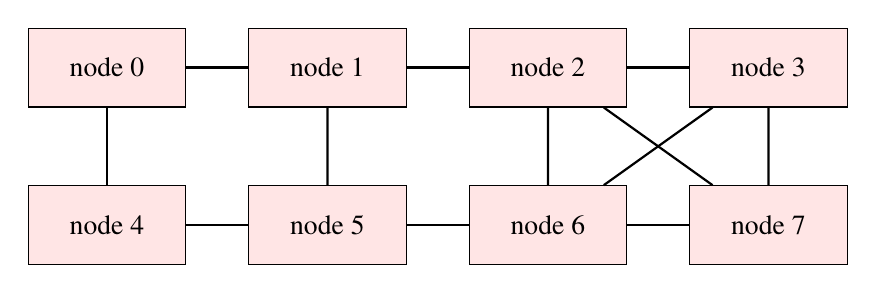
\begin{tikzpicture}[
    xscale=.7,
    yscale=.5,
    every node/.style={draw,fill=red!10,minimum width=2cm,minimum height=1cm}
    ]
    \node (c1) at ( 0, 4) {node 0};
    \node (c2) at ( 4, 4) {node 1};
    \node (c3) at ( 8, 4) {node 2};
    \node (c4) at (12, 4) {node 3};

    \node (c5) at ( 0, 0) {node 4};
    \node (c6) at ( 4, 0) {node 5};
    \node (c7) at ( 8, 0) {node 6};
    \node (c8) at (12, 0) {node 7};

    % top horizontal
    \draw[thick] (c1) -- (c2);
    \draw[thick] (c2) -- (c3);
    \draw[thick] (c3) -- (c4);
    % bottom horizontal
    \draw[thick] (c5) -- (c6);
    \draw[thick] (c6) -- (c7);
    \draw[thick] (c7) -- (c8);
    % vertical
    \draw[thick] (c1) -- (c5);
    \draw[thick] (c2) -- (c6);
    \draw[thick] (c3) -- (c7);
    \draw[thick] (c4) -- (c8);
    % cross
    \draw[thick] (c3) -- (c8);
    \draw[thick] (c4) -- (c7);
  \end{tikzpicture}
  \caption{Interconnect topology of 8x4x1 AMD Shanghai machine}
  \label{fig:gruyere}
\end{figure}

%%%%%%%%%%%%%%%%%%%%%%%%%%%%%%%%%%%%%%%%%%%%%%%%%%
% Example: Atomic broadcast
%%%%%%%%%%%%%%%%%%%%%%%%%%%%%%%%%%%%%%%%%%%%%%%%%%
\section{Atomic Broadcast}

We build our atomic broadcast based on an overlay network connecting
all nodes of a given multicore machine. 

As a first step, we evaluate tree based overlay networks. Other
potentially interesting topologies are rings.

%%%%%%%%%%%%%%%%%%%%%%%%%%%%%%%%%%%%%%%%%%%%%%%%%%
\subsection{Tree}

We now look at tree based atomic broadcast implementations. 

The first challenge is to find efficient spanning trees for arbitrary
machines. These machines are represented by a model, which we
described earlier.

%%%%%%%%%%%%%%%%%%%%%%%%%%%%%%%%%%%%%%%%%%%%%%%%%%
\subsubsection{Divide and conquer}

We divide the space into clusters. In every round, we further split up
all cluster into smaller clusters and connect them with the minimal
link. 

We find this link by searching for links that have start and
end node in different regions of the most recent split. Out of these
links, we pick the cheapest ones. We ignore links whose start or end
node have a too high degree in the spanning tree already.

Assuming that the choice of node IDs represents the topology to some
extend, splitting them up into distinct clusters avoids contention, as
two separate sub-trees are processed in different areas of the
interconnect network.

%%%%%%%%%%%%%%%%%%%%%%%%%%%%%%%%%%%%%%%%%%%%%%%%%%
\subsubsection{Clustering}

Another idea is to employ clustering. One example is to base this on
NUMA domains such that every NUMA domain corresponds to one cluster. 

%%%%%%%%%%%%%%%%%%%%%%%%%%%%%%%%%%%%%%%%%%%%%%%%%%
\subsubsection{Minimum-Spanning Tree}

We can apply a minimum spanning tree algorithm to the machine model
graph to find a number of links such that these links connect all
nodes at a minimum cost.

We have implemented such an algorithm and found out, that it is not a
good solution in the general case, since it does not consider
parallelism. Naturally, we would like to parallelize send operations
to different nodes, which allows them to send messages in parallel. 

An example is obvious in Figure~\ref{fig:mst_gruyere_operations}. The
level of parallelism is only two. Cores 00 to 15 are dealt with in
parallel to cores 16 to 31. Other than that, there is no further
parallelism although it is possible to ``split up'' communication with
every new ``round'' (i.e.\ send operations of nodes).

An important variable in constructing such a tree is the degree of
nodes. If the send cost $t_s$ is smaller than the propagation time
$t_p$,  $d = \lfloor \frac{t_p}{t_s} \rfloor$ messages can be send to
hide propagation of messages. Hence, a tree with degree $d$ should be
ideal to minimize latency, but only for an acknowledged protocol.

%%%%%%%%%%%%%%%%%%%%%%%%%%%%%%%%%%%%%%%%%%%%%%%%%%
\subsection{Scheduling}

% Tree -> scheduling
Assuming the tree (or some other kind of overlay network), there is a
\emph{scheduling problems} for the order in which to send messages to
children. The intuition is to send on long-delay links first to hide
the more expensive latencies, as this link is dominating total send
cost.

We show an example of bad scheduling in
Figure~\ref{fig:mst_gruyere_operations}. When core 08 sends its six
messages, it does so in naive order (here: in increasing node ID
order). This is inefficient, as the latency of the broadcast is
dominated by cores 12, 24 and 28 rather than cores 9, 10 and 11. A
better schedule for sending messages to the children of core 8 would
be to start with the child from which the longest path emerges.

%%%%%%%%%%%%%%%%%%%%%%%%%%%%%%%%%%%%%%%%%%%%%%%%%%
\subsection{Example tree}

We show the multicast tree automatically generated from a fully meshed
machine model of a 8x4x1 sample multicore (gruyere) in
Figure~\ref{fig:mst_gruyere}. We get this tree by applying a minimum
spanning tree algorithm on a multicore model encoding link latencies.

\begin{figure}
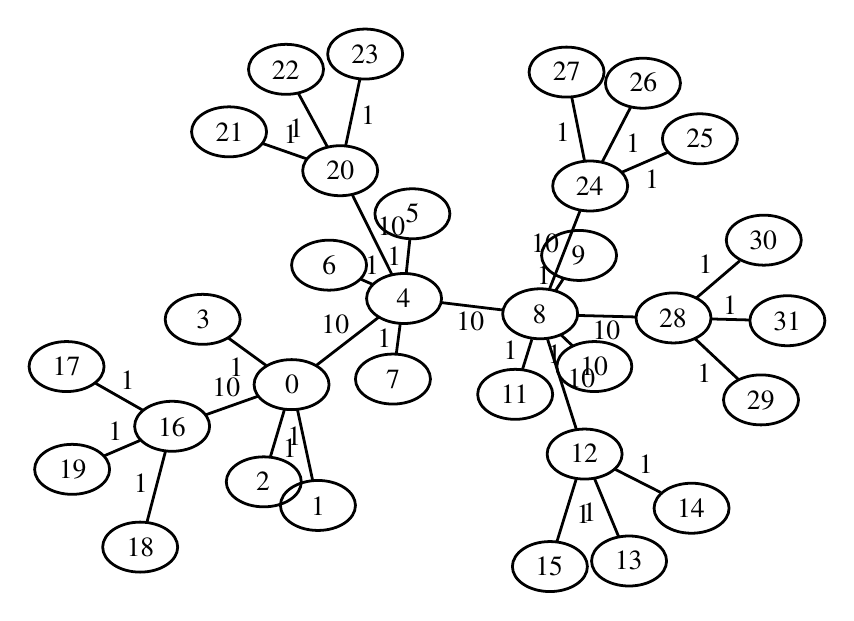
\begin{tikzpicture}[>=latex,line join=bevel,scale=.5]
  \pgfsetlinewidth{1bp}
%%
\pgfsetcolor{black}
  % Edge: 0 -- 16
  \draw [] (166.21bp,141.75bp) .. controls (154.21bp,137.5bp) and (139.75bp,132.37bp)  .. (127.78bp,128.12bp);
  \definecolor{strokecol}{rgb}{0.0,0.0,0.0};
  \pgfsetstrokecolor{strokecol}
  \draw (142.99bp,147.94bp) node {$10$};
  % Edge: 24 -- 8
  \draw [] (397.66bp,275.03bp) .. controls (391.25bp,258.58bp) and (381.78bp,234.27bp)  .. (375.41bp,217.94bp);
  \draw (372.53bp,251.48bp) node {$10$};
  % Edge: 3 -- 0
  \draw [] (144.86bp,183.29bp) .. controls (153.27bp,177.19bp) and (163.2bp,169.98bp)  .. (171.63bp,163.85bp);
  \draw (150.24bp,162.57bp) node {$1$};
  % Edge: 13 -- 12
  \draw [] (425.39bp,40.785bp) .. controls (420.15bp,53.394bp) and (413.1bp,70.342bp)  .. (407.87bp,82.936bp);
  \draw (404.63bp,57.86bp) node {$1$};
  % Edge: 28 -- 30
  \draw [] (481.35bp,212.31bp) .. controls (490.97bp,220.54bp) and (503.03bp,230.85bp)  .. (512.69bp,239.11bp);
  \draw (488.02bp,236.71bp) node {$1$};
  % Edge: 20 -- 21
  \draw [] (201.17bp,312.44bp) .. controls (191.17bp,315.94bp) and (179.56bp,319.99bp)  .. (169.53bp,323.49bp);
  \draw (189.35bp,329.97bp) node {$1$};
  % Edge: 14 -- 12
  \draw [] (455.7bp,72.393bp) .. controls (445.22bp,77.713bp) and (432.7bp,84.068bp)  .. (422.25bp,89.375bp);
  \draw (444.97bp,92.884bp) node {$1$};
  % Edge: 24 -- 25
  \draw [] (427.6bp,302.81bp) .. controls (438.25bp,307.43bp) and (450.85bp,312.89bp)  .. (461.46bp,317.49bp);
  \draw (449.53bp,298.15bp) node {$1$};
  % Edge: 23 -- 20
  \draw [] (239.16bp,369.78bp) .. controls (236.13bp,355.61bp) and (231.94bp,336.05bp)  .. (228.93bp,321.97bp);
  \draw (245.04bp,343.88bp) node {$1$};
  % Edge: 10 -- 8
  \draw [] (392.35bp,177.85bp) .. controls (389.69bp,180.39bp) and (386.93bp,183.02bp)  .. (384.27bp,185.56bp);
  \draw (379.31bp,171.71bp) node {$1$};
  % Edge: 28 -- 29
  \draw [] (480.24bp,183.31bp) .. controls (489.9bp,174.24bp) and (502.25bp,162.63bp)  .. (511.95bp,153.51bp);
  \draw (487.09bp,158.41bp) node {$1$};
  % Edge: 9 -- 8
  \draw [] (385.56bp,225.98bp) .. controls (383.61bp,223.03bp) and (381.57bp,219.97bp)  .. (379.61bp,217.03bp);
  \draw (371.59bp,228.5bp) node {$1$};
  % Edge: 26 -- 24
  \draw [] (434.35bp,350.12bp) .. controls (428.09bp,338.07bp) and (419.78bp,322.07bp)  .. (413.53bp,310.04bp);
  \draw (435.94bp,324.08bp) node {$1$};
  % Edge: 8 -- 11
  \draw [] (363.03bp,182.61bp) .. controls (360.85bp,175.62bp) and (358.35bp,167.62bp)  .. (356.17bp,160.64bp);
  \draw (347.6bp,174.63bp) node {$1$};
  % Edge: 6 -- 4
  \draw [] (239.87bp,225.9bp) .. controls (242.6bp,224.69bp) and (245.39bp,223.47bp)  .. (248.12bp,222.27bp);
  \draw (247.99bp,236.08bp) node {$1$};
  % Edge: 15 -- 12
  \draw [] (380.96bp,36.652bp) .. controls (385.14bp,50.203bp) and (390.9bp,68.839bp)  .. (395.1bp,82.452bp);
  \draw (400.03bp,56.552bp) node {$1$};
  % Edge: 20 -- 4
  \draw [] (233.67bp,286.83bp) .. controls (241.82bp,270.43bp) and (254bp,245.9bp)  .. (262.13bp,229.53bp);
  \draw (261.9bp,264.18bp) node {$10$};
  % Edge: 18 -- 16
  \draw [] (85.864bp,50.894bp) .. controls (89.75bp,65.773bp) and (95.245bp,86.812bp)  .. (99.13bp,101.68bp);
  \draw (81.497bp,79.29bp) node {$1$};
  % Edge: 27 -- 24
  \draw [] (391.64bp,357.44bp) .. controls (394.41bp,343.6bp) and (398.24bp,324.53bp)  .. (401.01bp,310.7bp);
  \draw (385.32bp,332.07bp) node {$1$};
  % Edge: 2 -- 0
  \draw [] (174.87bp,98.4bp) .. controls (178bp,108.92bp) and (181.93bp,122.13bp)  .. (185.04bp,132.6bp);
  \draw (191.95bp,112.5bp) node {$1$};
  % Edge: 28 -- 8
  \draw [] (437.62bp,198.71bp) .. controls (424.53bp,199.05bp) and (408.85bp,199.46bp)  .. (395.75bp,199.8bp);
  \draw (416.68bp,189.25bp) node {$10$};
  % Edge: 19 -- 16
  \draw [] (55.352bp,98.839bp) .. controls (63.514bp,102.34bp) and (72.694bp,106.28bp)  .. (80.851bp,109.78bp);
  \draw (63.102bp,116.31bp) node {$1$};
  % Edge: 4 -- 0
  \draw [] (252.83bp,198.58bp) .. controls (239.51bp,188.29bp) and (221.39bp,174.3bp)  .. (208.08bp,164.03bp);
  \draw (221.46bp,193.3bp) node {$10$};
  % Edge: 8 -- 12
  \draw [] (374.34bp,182.6bp) .. controls (380.17bp,164.37bp) and (389.15bp,136.27bp)  .. (394.96bp,118.1bp);
  \draw (398.65bp,154.35bp) node {$10$};
  % Edge: 20 -- 22
  \draw [] (215.78bp,321.25bp) .. controls (209.51bp,332.8bp) and (201.28bp,347.96bp)  .. (195.03bp,359.48bp);
  \draw (193.4bp,334.37bp) node {$1$};
  % Edge: 1 -- 0
  \draw [] (205.21bp,80.92bp) .. controls (201.98bp,95.938bp) and (197.42bp,117.17bp)  .. (194.19bp,132.19bp);
  \draw (188.7bp,104.55bp) node {$1$};
  % Edge: 4 -- 8
  \draw [] (297.43bp,209.11bp) .. controls (311.25bp,207.44bp) and (328.07bp,205.41bp)  .. (341.89bp,203.74bp);
  \draw (318.66bp,195.43bp) node {$10$};
  % Edge: 17 -- 16
  \draw [] (48.717bp,151.05bp) .. controls (59.414bp,144.95bp) and (72.429bp,137.53bp)  .. (83.123bp,131.43bp);
  \draw (71.92bp,153.24bp) node {$1$};
  % Edge: 4 -- 7
  \draw [] (268.29bp,194.2bp) .. controls (267.36bp,187.11bp) and (266.29bp,178.99bp)  .. (265.36bp,171.91bp);
  \draw (256.82bp,183.06bp) node {$1$};
  % Edge: 5 -- 4
  \draw [] (275.2bp,254.93bp) .. controls (274.38bp,247.23bp) and (273.43bp,238.29bp)  .. (272.61bp,230.59bp);
  \draw (263.9bp,242.76bp) node {$1$};
  % Edge: 28 -- 31
  \draw [] (492bp,197.27bp) .. controls (500.87bp,197.04bp) and (510.71bp,196.77bp)  .. (519.58bp,196.54bp);
  \draw (505.79bp,206.91bp) node {$1$};
  % Node: 24
\begin{scope}
  \definecolor{strokecol}{rgb}{0.0,0.0,0.0};
  \pgfsetstrokecolor{strokecol}
  \draw (405bp,293bp) ellipse (27bp and 18bp);
  \draw (404.59bp,292.83bp) node {$24$};
\end{scope}
  % Node: 25
\begin{scope}
  \definecolor{strokecol}{rgb}{0.0,0.0,0.0};
  \pgfsetstrokecolor{strokecol}
  \draw (484bp,327bp) ellipse (27bp and 18bp);
  \draw (484.14bp,327.33bp) node {$25$};
\end{scope}
  % Node: 26
\begin{scope}
  \definecolor{strokecol}{rgb}{0.0,0.0,0.0};
  \pgfsetstrokecolor{strokecol}
  \draw (443bp,367bp) ellipse (27bp and 18bp);
  \draw (443.33bp,367.42bp) node {$26$};
\end{scope}
  % Node: 27
\begin{scope}
  \definecolor{strokecol}{rgb}{0.0,0.0,0.0};
  \pgfsetstrokecolor{strokecol}
  \draw (388bp,375bp) ellipse (27bp and 18bp);
  \draw (388.04bp,375.34bp) node {$27$};
\end{scope}
  % Node: 20
\begin{scope}
  \definecolor{strokecol}{rgb}{0.0,0.0,0.0};
  \pgfsetstrokecolor{strokecol}
  \draw (225bp,304bp) ellipse (27bp and 18bp);
  \draw (225.1bp,304.09bp) node {$20$};
\end{scope}
  % Node: 21
\begin{scope}
  \definecolor{strokecol}{rgb}{0.0,0.0,0.0};
  \pgfsetstrokecolor{strokecol}
  \draw (145bp,332bp) ellipse (27bp and 18bp);
  \draw (145.34bp,331.94bp) node {$21$};
\end{scope}
  % Node: 22
\begin{scope}
  \definecolor{strokecol}{rgb}{0.0,0.0,0.0};
  \pgfsetstrokecolor{strokecol}
  \draw (186bp,377bp) ellipse (27bp and 18bp);
  \draw (185.78bp,376.53bp) node {$22$};
\end{scope}
  % Node: 23
\begin{scope}
  \definecolor{strokecol}{rgb}{0.0,0.0,0.0};
  \pgfsetstrokecolor{strokecol}
  \draw (243bp,388bp) ellipse (27bp and 18bp);
  \draw (243.05bp,387.99bp) node {$23$};
\end{scope}
  % Node: 28
\begin{scope}
  \definecolor{strokecol}{rgb}{0.0,0.0,0.0};
  \pgfsetstrokecolor{strokecol}
  \draw (465bp,198bp) ellipse (27bp and 18bp);
  \draw (464.62bp,198bp) node {$28$};
\end{scope}
  % Node: 29
\begin{scope}
  \definecolor{strokecol}{rgb}{0.0,0.0,0.0};
  \pgfsetstrokecolor{strokecol}
  \draw (528bp,139bp) ellipse (27bp and 18bp);
  \draw (527.83bp,138.57bp) node {$29$};
\end{scope}
  % Node: 1
\begin{scope}
  \definecolor{strokecol}{rgb}{0.0,0.0,0.0};
  \pgfsetstrokecolor{strokecol}
  \draw (209bp,63bp) ellipse (27bp and 18bp);
  \draw (209.11bp,62.79bp) node {$1$};
\end{scope}
  % Node: 0
\begin{scope}
  \definecolor{strokecol}{rgb}{0.0,0.0,0.0};
  \pgfsetstrokecolor{strokecol}
  \draw (190bp,150bp) ellipse (27bp and 18bp);
  \draw (190.3bp,150.29bp) node {$0$};
\end{scope}
  % Node: 3
\begin{scope}
  \definecolor{strokecol}{rgb}{0.0,0.0,0.0};
  \pgfsetstrokecolor{strokecol}
  \draw (126bp,197bp) ellipse (27bp and 18bp);
  \draw (126.37bp,196.72bp) node {$3$};
\end{scope}
  % Node: 2
\begin{scope}
  \definecolor{strokecol}{rgb}{0.0,0.0,0.0};
  \pgfsetstrokecolor{strokecol}
  \draw (170bp,80bp) ellipse (27bp and 18bp);
  \draw (169.52bp,80.402bp) node {$2$};
\end{scope}
  % Node: 5
\begin{scope}
  \definecolor{strokecol}{rgb}{0.0,0.0,0.0};
  \pgfsetstrokecolor{strokecol}
  \draw (277bp,273bp) ellipse (27bp and 18bp);
  \draw (277.14bp,273.19bp) node {$5$};
\end{scope}
  % Node: 4
\begin{scope}
  \definecolor{strokecol}{rgb}{0.0,0.0,0.0};
  \pgfsetstrokecolor{strokecol}
  \draw (271bp,212bp) ellipse (27bp and 18bp);
  \draw (270.67bp,212.35bp) node {$4$};
\end{scope}
  % Node: 7
\begin{scope}
  \definecolor{strokecol}{rgb}{0.0,0.0,0.0};
  \pgfsetstrokecolor{strokecol}
  \draw (263bp,154bp) ellipse (27bp and 18bp);
  \draw (263.01bp,153.98bp) node {$7$};
\end{scope}
  % Node: 6
\begin{scope}
  \definecolor{strokecol}{rgb}{0.0,0.0,0.0};
  \pgfsetstrokecolor{strokecol}
  \draw (217bp,236bp) ellipse (27bp and 18bp);
  \draw (217.18bp,235.87bp) node {$6$};
\end{scope}
  % Node: 9
\begin{scope}
  \definecolor{strokecol}{rgb}{0.0,0.0,0.0};
  \pgfsetstrokecolor{strokecol}
  \draw (397bp,243bp) ellipse (27bp and 18bp);
  \draw (396.64bp,242.62bp) node {$9$};
\end{scope}
  % Node: 8
\begin{scope}
  \definecolor{strokecol}{rgb}{0.0,0.0,0.0};
  \pgfsetstrokecolor{strokecol}
  \draw (369bp,201bp) ellipse (27bp and 18bp);
  \draw (368.62bp,200.5bp) node {$8$};
\end{scope}
  % Node: 11
\begin{scope}
  \definecolor{strokecol}{rgb}{0.0,0.0,0.0};
  \pgfsetstrokecolor{strokecol}
  \draw (351bp,143bp) ellipse (27bp and 18bp);
  \draw (350.65bp,142.96bp) node {$11$};
\end{scope}
  % Node: 10
\begin{scope}
  \definecolor{strokecol}{rgb}{0.0,0.0,0.0};
  \pgfsetstrokecolor{strokecol}
  \draw (408bp,163bp) ellipse (27bp and 18bp);
  \draw (407.85bp,163.05bp) node {$10$};
\end{scope}
  % Node: 13
\begin{scope}
  \definecolor{strokecol}{rgb}{0.0,0.0,0.0};
  \pgfsetstrokecolor{strokecol}
  \draw (433bp,23bp) ellipse (27bp and 18bp);
  \draw (432.66bp,23.301bp) node {$13$};
\end{scope}
  % Node: 12
\begin{scope}
  \definecolor{strokecol}{rgb}{0.0,0.0,0.0};
  \pgfsetstrokecolor{strokecol}
  \draw (401bp,100bp) ellipse (27bp and 18bp);
  \draw (400.63bp,100.35bp) node {$12$};
\end{scope}
  % Node: 15
\begin{scope}
  \definecolor{strokecol}{rgb}{0.0,0.0,0.0};
  \pgfsetstrokecolor{strokecol}
  \draw (376bp,19bp) ellipse (27bp and 18bp);
  \draw (375.51bp,19bp) node {$15$};
\end{scope}
  % Node: 14
\begin{scope}
  \definecolor{strokecol}{rgb}{0.0,0.0,0.0};
  \pgfsetstrokecolor{strokecol}
  \draw (478bp,61bp) ellipse (27bp and 18bp);
  \draw (477.53bp,61.31bp) node {$14$};
\end{scope}
  % Node: 17
\begin{scope}
  \definecolor{strokecol}{rgb}{0.0,0.0,0.0};
  \pgfsetstrokecolor{strokecol}
  \draw (28bp,163bp) ellipse (27bp and 18bp);
  \draw (28bp,162.87bp) node {$17$};
\end{scope}
  % Node: 16
\begin{scope}
  \definecolor{strokecol}{rgb}{0.0,0.0,0.0};
  \pgfsetstrokecolor{strokecol}
  \draw (104bp,120bp) ellipse (27bp and 18bp);
  \draw (103.82bp,119.62bp) node {$16$};
\end{scope}
  % Node: 19
\begin{scope}
  \definecolor{strokecol}{rgb}{0.0,0.0,0.0};
  \pgfsetstrokecolor{strokecol}
  \draw (32bp,89bp) ellipse (27bp and 18bp);
  \draw (32.345bp,88.971bp) node {$19$};
\end{scope}
  % Node: 18
\begin{scope}
  \definecolor{strokecol}{rgb}{0.0,0.0,0.0};
  \pgfsetstrokecolor{strokecol}
  \draw (81bp,33bp) ellipse (27bp and 18bp);
  \draw (81.173bp,32.931bp) node {$18$};
\end{scope}
  % Node: 31
\begin{scope}
  \definecolor{strokecol}{rgb}{0.0,0.0,0.0};
  \pgfsetstrokecolor{strokecol}
  \draw (547bp,196bp) ellipse (27bp and 18bp);
  \draw (546.84bp,195.81bp) node {$31$};
\end{scope}
  % Node: 30
\begin{scope}
  \definecolor{strokecol}{rgb}{0.0,0.0,0.0};
  \pgfsetstrokecolor{strokecol}
  \draw (530bp,254bp) ellipse (27bp and 18bp);
  \draw (529.59bp,253.56bp) node {$30$};
\end{scope}
%

\end{tikzpicture}
\caption{Multicast tree automatically found for a 8x4x1 multicore}
\label{fig:mst_gruyere}
\end{figure}

In Figure~\ref{fig:mst_gruyere_operations}, we show the order of
operations for sending a broadcast message along the MST given in
Figure~\ref{fig:mst_gruyere}. 

\begin{figure}[htb]
  \centering
  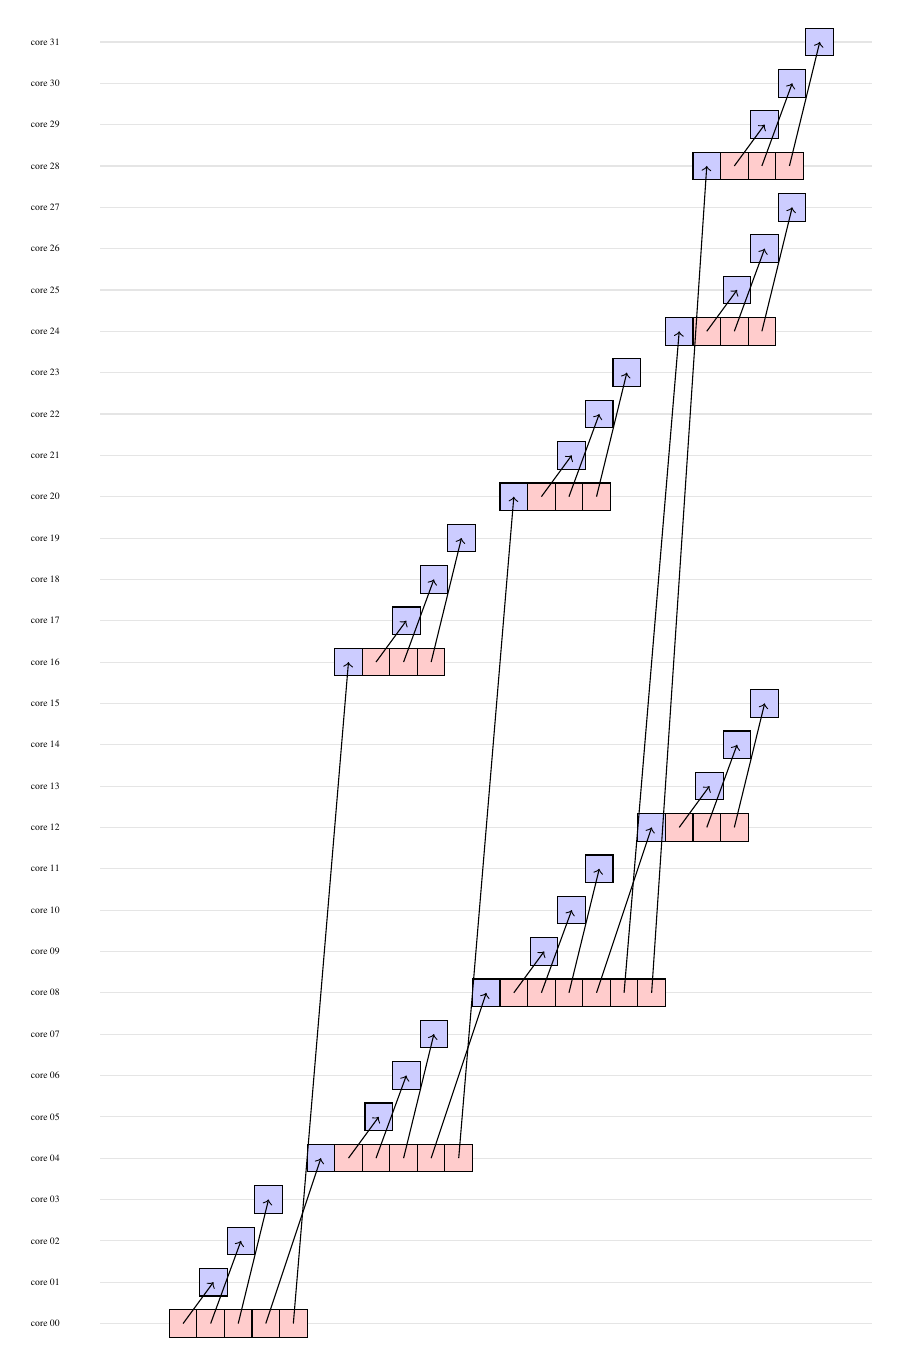
\begin{tikzpicture}[scale=.35,transform shape]
    % Insert visualization
    \node at (0mm,0mm) {core 00};
\draw[color=black!10] (20mm,0mm) -- (30cm,0mm);
\node at (0mm,15mm) {core 01};
\draw[color=black!10] (20mm,15mm) -- (30cm,15mm);
\node at (0mm,30mm) {core 02};
\draw[color=black!10] (20mm,30mm) -- (30cm,30mm);
\node at (0mm,45mm) {core 03};
\draw[color=black!10] (20mm,45mm) -- (30cm,45mm);
\node at (0mm,60mm) {core 04};
\draw[color=black!10] (20mm,60mm) -- (30cm,60mm);
\node at (0mm,75mm) {core 05};
\draw[color=black!10] (20mm,75mm) -- (30cm,75mm);
\node at (0mm,90mm) {core 06};
\draw[color=black!10] (20mm,90mm) -- (30cm,90mm);
\node at (0mm,105mm) {core 07};
\draw[color=black!10] (20mm,105mm) -- (30cm,105mm);
\node at (0mm,120mm) {core 08};
\draw[color=black!10] (20mm,120mm) -- (30cm,120mm);
\node at (0mm,135mm) {core 09};
\draw[color=black!10] (20mm,135mm) -- (30cm,135mm);
\node at (0mm,150mm) {core 10};
\draw[color=black!10] (20mm,150mm) -- (30cm,150mm);
\node at (0mm,165mm) {core 11};
\draw[color=black!10] (20mm,165mm) -- (30cm,165mm);
\node at (0mm,180mm) {core 12};
\draw[color=black!10] (20mm,180mm) -- (30cm,180mm);
\node at (0mm,195mm) {core 13};
\draw[color=black!10] (20mm,195mm) -- (30cm,195mm);
\node at (0mm,210mm) {core 14};
\draw[color=black!10] (20mm,210mm) -- (30cm,210mm);
\node at (0mm,225mm) {core 15};
\draw[color=black!10] (20mm,225mm) -- (30cm,225mm);
\node at (0mm,240mm) {core 16};
\draw[color=black!10] (20mm,240mm) -- (30cm,240mm);
\node at (0mm,255mm) {core 17};
\draw[color=black!10] (20mm,255mm) -- (30cm,255mm);
\node at (0mm,270mm) {core 18};
\draw[color=black!10] (20mm,270mm) -- (30cm,270mm);
\node at (0mm,285mm) {core 19};
\draw[color=black!10] (20mm,285mm) -- (30cm,285mm);
\node at (0mm,300mm) {core 20};
\draw[color=black!10] (20mm,300mm) -- (30cm,300mm);
\node at (0mm,315mm) {core 21};
\draw[color=black!10] (20mm,315mm) -- (30cm,315mm);
\node at (0mm,330mm) {core 22};
\draw[color=black!10] (20mm,330mm) -- (30cm,330mm);
\node at (0mm,345mm) {core 23};
\draw[color=black!10] (20mm,345mm) -- (30cm,345mm);
\node at (0mm,360mm) {core 24};
\draw[color=black!10] (20mm,360mm) -- (30cm,360mm);
\node at (0mm,375mm) {core 25};
\draw[color=black!10] (20mm,375mm) -- (30cm,375mm);
\node at (0mm,390mm) {core 26};
\draw[color=black!10] (20mm,390mm) -- (30cm,390mm);
\node at (0mm,405mm) {core 27};
\draw[color=black!10] (20mm,405mm) -- (30cm,405mm);
\node at (0mm,420mm) {core 28};
\draw[color=black!10] (20mm,420mm) -- (30cm,420mm);
\node at (0mm,435mm) {core 29};
\draw[color=black!10] (20mm,435mm) -- (30cm,435mm);
\node at (0mm,450mm) {core 30};
\draw[color=black!10] (20mm,450mm) -- (30cm,450mm);
\node at (0mm,465mm) {core 31};
\draw[color=black!10] (20mm,465mm) -- (30cm,465mm);
\node[draw,fill=red!20,minimum size=10mm] (s_0_1) at (50mm,0mm) {};
\node[draw,fill=red!20,minimum size=10mm] (s_0_2) at (60mm,0mm) {};
\node[draw,fill=red!20,minimum size=10mm] (s_0_3) at (70mm,0mm) {};
\node[draw,fill=red!20,minimum size=10mm] (s_0_4) at (80mm,0mm) {};
\node[draw,fill=red!20,minimum size=10mm] (s_0_16) at (90mm,0mm) {};
\node[draw,fill=blue!20,minimum size=10mm] (r_0_1) at (61mm,15mm) {};
\draw[->] (s_0_1.center) -- (r_0_1.center); 
\node[draw,fill=blue!20,minimum size=10mm] (r_0_2) at (71mm,30mm) {};
\draw[->] (s_0_2.center) -- (r_0_2.center); 
\node[draw,fill=blue!20,minimum size=10mm] (r_0_3) at (81mm,45mm) {};
\draw[->] (s_0_3.center) -- (r_0_3.center); 
\node[draw,fill=blue!20,minimum size=10mm] (r_0_4) at (100mm,60mm) {};
\draw[->] (s_0_4.center) -- (r_0_4.center); 
\node[draw,fill=red!20,minimum size=10mm] (s_4_5) at (110mm,60mm) {};
\node[draw,fill=red!20,minimum size=10mm] (s_4_6) at (120mm,60mm) {};
\node[draw,fill=red!20,minimum size=10mm] (s_4_7) at (130mm,60mm) {};
\node[draw,fill=red!20,minimum size=10mm] (s_4_8) at (140mm,60mm) {};
\node[draw,fill=red!20,minimum size=10mm] (s_4_20) at (150mm,60mm) {};
\node[draw,fill=blue!20,minimum size=10mm] (r_0_16) at (110mm,240mm) {};
\draw[->] (s_0_16.center) -- (r_0_16.center); 
\node[draw,fill=red!20,minimum size=10mm] (s_16_17) at (120mm,240mm) {};
\node[draw,fill=red!20,minimum size=10mm] (s_16_18) at (130mm,240mm) {};
\node[draw,fill=red!20,minimum size=10mm] (s_16_19) at (140mm,240mm) {};
\node[draw,fill=blue!20,minimum size=10mm] (r_4_5) at (121mm,75mm) {};
\draw[->] (s_4_5.center) -- (r_4_5.center); 
\node[draw,fill=blue!20,minimum size=10mm] (r_16_17) at (131mm,255mm) {};
\draw[->] (s_16_17.center) -- (r_16_17.center); 
\node[draw,fill=blue!20,minimum size=10mm] (r_4_6) at (131mm,90mm) {};
\draw[->] (s_4_6.center) -- (r_4_6.center); 
\node[draw,fill=blue!20,minimum size=10mm] (r_16_18) at (141mm,270mm) {};
\draw[->] (s_16_18.center) -- (r_16_18.center); 
\node[draw,fill=blue!20,minimum size=10mm] (r_4_7) at (141mm,105mm) {};
\draw[->] (s_4_7.center) -- (r_4_7.center); 
\node[draw,fill=blue!20,minimum size=10mm] (r_16_19) at (151mm,285mm) {};
\draw[->] (s_16_19.center) -- (r_16_19.center); 
\node[draw,fill=blue!20,minimum size=10mm] (r_4_8) at (160mm,120mm) {};
\draw[->] (s_4_8.center) -- (r_4_8.center); 
\node[draw,fill=red!20,minimum size=10mm] (s_8_9) at (170mm,120mm) {};
\node[draw,fill=red!20,minimum size=10mm] (s_8_10) at (180mm,120mm) {};
\node[draw,fill=red!20,minimum size=10mm] (s_8_11) at (190mm,120mm) {};
\node[draw,fill=red!20,minimum size=10mm] (s_8_12) at (200mm,120mm) {};
\node[draw,fill=red!20,minimum size=10mm] (s_8_24) at (210mm,120mm) {};
\node[draw,fill=red!20,minimum size=10mm] (s_8_28) at (220mm,120mm) {};
\node[draw,fill=blue!20,minimum size=10mm] (r_4_20) at (170mm,300mm) {};
\draw[->] (s_4_20.center) -- (r_4_20.center); 
\node[draw,fill=red!20,minimum size=10mm] (s_20_21) at (180mm,300mm) {};
\node[draw,fill=red!20,minimum size=10mm] (s_20_22) at (190mm,300mm) {};
\node[draw,fill=red!20,minimum size=10mm] (s_20_23) at (200mm,300mm) {};
\node[draw,fill=blue!20,minimum size=10mm] (r_8_9) at (181mm,135mm) {};
\draw[->] (s_8_9.center) -- (r_8_9.center); 
\node[draw,fill=blue!20,minimum size=10mm] (r_20_21) at (191mm,315mm) {};
\draw[->] (s_20_21.center) -- (r_20_21.center); 
\node[draw,fill=blue!20,minimum size=10mm] (r_8_10) at (191mm,150mm) {};
\draw[->] (s_8_10.center) -- (r_8_10.center); 
\node[draw,fill=blue!20,minimum size=10mm] (r_20_22) at (201mm,330mm) {};
\draw[->] (s_20_22.center) -- (r_20_22.center); 
\node[draw,fill=blue!20,minimum size=10mm] (r_8_11) at (201mm,165mm) {};
\draw[->] (s_8_11.center) -- (r_8_11.center); 
\node[draw,fill=blue!20,minimum size=10mm] (r_20_23) at (211mm,345mm) {};
\draw[->] (s_20_23.center) -- (r_20_23.center); 
\node[draw,fill=blue!20,minimum size=10mm] (r_8_12) at (220mm,180mm) {};
\draw[->] (s_8_12.center) -- (r_8_12.center); 
\node[draw,fill=red!20,minimum size=10mm] (s_12_13) at (230mm,180mm) {};
\node[draw,fill=red!20,minimum size=10mm] (s_12_14) at (240mm,180mm) {};
\node[draw,fill=red!20,minimum size=10mm] (s_12_15) at (250mm,180mm) {};
\node[draw,fill=blue!20,minimum size=10mm] (r_8_24) at (230mm,360mm) {};
\draw[->] (s_8_24.center) -- (r_8_24.center); 
\node[draw,fill=red!20,minimum size=10mm] (s_24_25) at (240mm,360mm) {};
\node[draw,fill=red!20,minimum size=10mm] (s_24_26) at (250mm,360mm) {};
\node[draw,fill=red!20,minimum size=10mm] (s_24_27) at (260mm,360mm) {};
\node[draw,fill=blue!20,minimum size=10mm] (r_8_28) at (240mm,420mm) {};
\draw[->] (s_8_28.center) -- (r_8_28.center); 
\node[draw,fill=red!20,minimum size=10mm] (s_28_29) at (250mm,420mm) {};
\node[draw,fill=red!20,minimum size=10mm] (s_28_30) at (260mm,420mm) {};
\node[draw,fill=red!20,minimum size=10mm] (s_28_31) at (270mm,420mm) {};
\node[draw,fill=blue!20,minimum size=10mm] (r_12_13) at (241mm,195mm) {};
\draw[->] (s_12_13.center) -- (r_12_13.center); 
\node[draw,fill=blue!20,minimum size=10mm] (r_12_14) at (251mm,210mm) {};
\draw[->] (s_12_14.center) -- (r_12_14.center); 
\node[draw,fill=blue!20,minimum size=10mm] (r_24_25) at (251mm,375mm) {};
\draw[->] (s_24_25.center) -- (r_24_25.center); 
\node[draw,fill=blue!20,minimum size=10mm] (r_28_29) at (261mm,435mm) {};
\draw[->] (s_28_29.center) -- (r_28_29.center); 
\node[draw,fill=blue!20,minimum size=10mm] (r_24_26) at (261mm,390mm) {};
\draw[->] (s_24_26.center) -- (r_24_26.center); 
\node[draw,fill=blue!20,minimum size=10mm] (r_12_15) at (261mm,225mm) {};
\draw[->] (s_12_15.center) -- (r_12_15.center); 
\node[draw,fill=blue!20,minimum size=10mm] (r_28_30) at (271mm,450mm) {};
\draw[->] (s_28_30.center) -- (r_28_30.center); 
\node[draw,fill=blue!20,minimum size=10mm] (r_24_27) at (271mm,405mm) {};
\draw[->] (s_24_27.center) -- (r_24_27.center); 
\node[draw,fill=blue!20,minimum size=10mm] (r_28_31) at (281mm,465mm) {};
\draw[->] (s_28_31.center) -- (r_28_31.center); 

  \end{tikzpicture}
  \caption{Visualization of operations for sending a message along the
    tree. Red boxes represent send operations, blue boxes represent
    receive operations and arrows messages sent between cores. The
    tree has been acquired using an MST algorithm.}
  \label{fig:mst_gruyere_operations}
\end{figure}

\begin{figure}[htb]
  \centering
  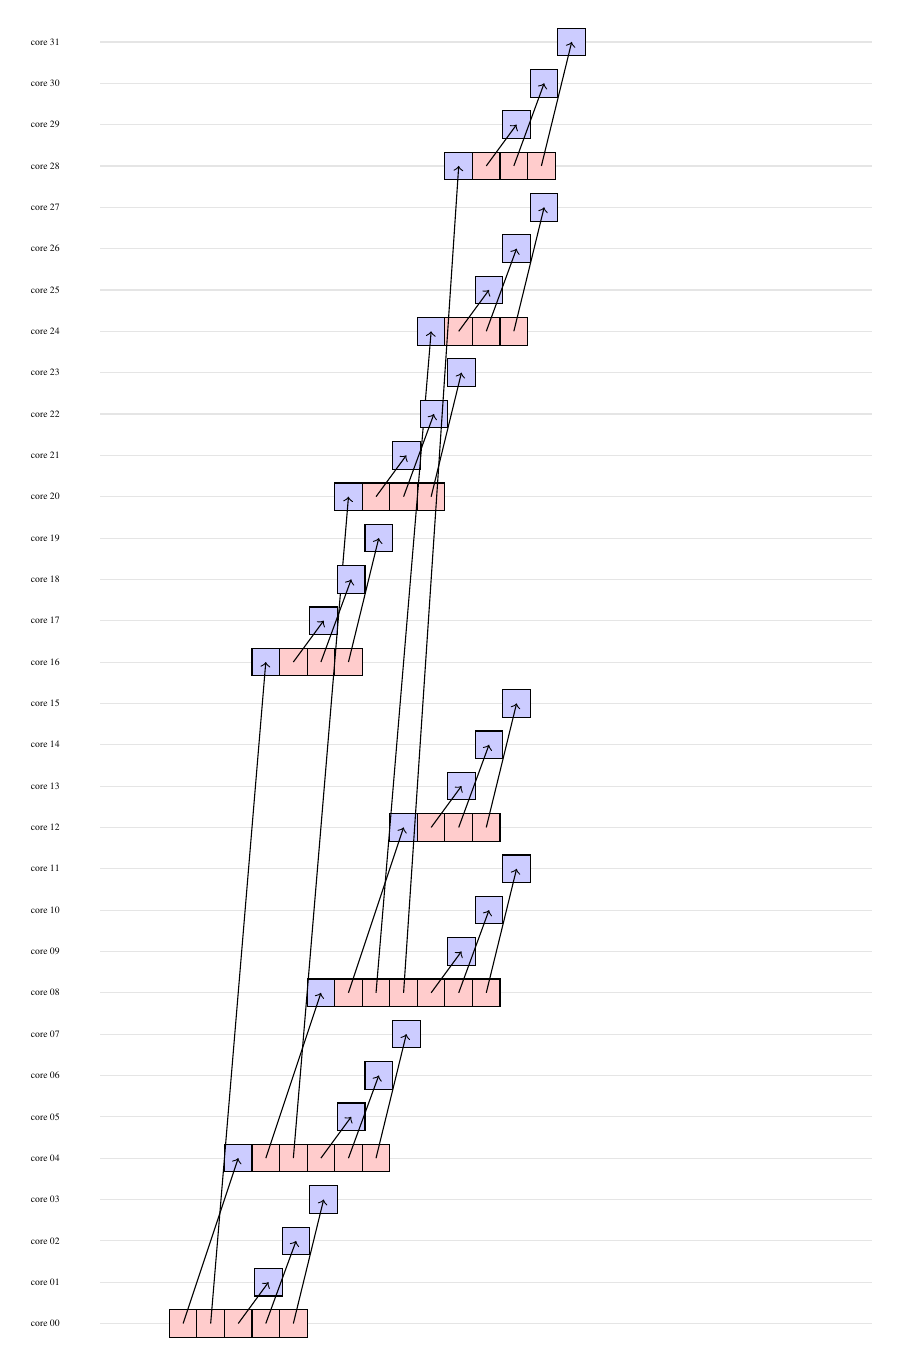
\begin{tikzpicture}[scale=.35,transform shape]
    % Insert visualization
    \node at (0mm,0mm) {core 00};
\draw[color=black!10] (20mm,0mm) -- (30cm,0mm);
\node at (0mm,15mm) {core 01};
\draw[color=black!10] (20mm,15mm) -- (30cm,15mm);
\node at (0mm,30mm) {core 02};
\draw[color=black!10] (20mm,30mm) -- (30cm,30mm);
\node at (0mm,45mm) {core 03};
\draw[color=black!10] (20mm,45mm) -- (30cm,45mm);
\node at (0mm,60mm) {core 04};
\draw[color=black!10] (20mm,60mm) -- (30cm,60mm);
\node at (0mm,75mm) {core 05};
\draw[color=black!10] (20mm,75mm) -- (30cm,75mm);
\node at (0mm,90mm) {core 06};
\draw[color=black!10] (20mm,90mm) -- (30cm,90mm);
\node at (0mm,105mm) {core 07};
\draw[color=black!10] (20mm,105mm) -- (30cm,105mm);
\node at (0mm,120mm) {core 08};
\draw[color=black!10] (20mm,120mm) -- (30cm,120mm);
\node at (0mm,135mm) {core 09};
\draw[color=black!10] (20mm,135mm) -- (30cm,135mm);
\node at (0mm,150mm) {core 10};
\draw[color=black!10] (20mm,150mm) -- (30cm,150mm);
\node at (0mm,165mm) {core 11};
\draw[color=black!10] (20mm,165mm) -- (30cm,165mm);
\node at (0mm,180mm) {core 12};
\draw[color=black!10] (20mm,180mm) -- (30cm,180mm);
\node at (0mm,195mm) {core 13};
\draw[color=black!10] (20mm,195mm) -- (30cm,195mm);
\node at (0mm,210mm) {core 14};
\draw[color=black!10] (20mm,210mm) -- (30cm,210mm);
\node at (0mm,225mm) {core 15};
\draw[color=black!10] (20mm,225mm) -- (30cm,225mm);
\node at (0mm,240mm) {core 16};
\draw[color=black!10] (20mm,240mm) -- (30cm,240mm);
\node at (0mm,255mm) {core 17};
\draw[color=black!10] (20mm,255mm) -- (30cm,255mm);
\node at (0mm,270mm) {core 18};
\draw[color=black!10] (20mm,270mm) -- (30cm,270mm);
\node at (0mm,285mm) {core 19};
\draw[color=black!10] (20mm,285mm) -- (30cm,285mm);
\node at (0mm,300mm) {core 20};
\draw[color=black!10] (20mm,300mm) -- (30cm,300mm);
\node at (0mm,315mm) {core 21};
\draw[color=black!10] (20mm,315mm) -- (30cm,315mm);
\node at (0mm,330mm) {core 22};
\draw[color=black!10] (20mm,330mm) -- (30cm,330mm);
\node at (0mm,345mm) {core 23};
\draw[color=black!10] (20mm,345mm) -- (30cm,345mm);
\node at (0mm,360mm) {core 24};
\draw[color=black!10] (20mm,360mm) -- (30cm,360mm);
\node at (0mm,375mm) {core 25};
\draw[color=black!10] (20mm,375mm) -- (30cm,375mm);
\node at (0mm,390mm) {core 26};
\draw[color=black!10] (20mm,390mm) -- (30cm,390mm);
\node at (0mm,405mm) {core 27};
\draw[color=black!10] (20mm,405mm) -- (30cm,405mm);
\node at (0mm,420mm) {core 28};
\draw[color=black!10] (20mm,420mm) -- (30cm,420mm);
\node at (0mm,435mm) {core 29};
\draw[color=black!10] (20mm,435mm) -- (30cm,435mm);
\node at (0mm,450mm) {core 30};
\draw[color=black!10] (20mm,450mm) -- (30cm,450mm);
\node at (0mm,465mm) {core 31};
\draw[color=black!10] (20mm,465mm) -- (30cm,465mm);
\node[draw,fill=red!20,minimum size=10mm] (s_0_4) at (50mm,0mm) {};
\node[draw,fill=red!20,minimum size=10mm] (s_0_16) at (60mm,0mm) {};
\node[draw,fill=red!20,minimum size=10mm] (s_0_1) at (70mm,0mm) {};
\node[draw,fill=red!20,minimum size=10mm] (s_0_2) at (80mm,0mm) {};
\node[draw,fill=red!20,minimum size=10mm] (s_0_3) at (90mm,0mm) {};
\node[draw,fill=blue!20,minimum size=10mm] (r_0_4) at (70mm,60mm) {};
\draw[->] (s_0_4.center) -- (r_0_4.center); 
\node[draw,fill=red!20,minimum size=10mm] (s_4_8) at (80mm,60mm) {};
\node[draw,fill=red!20,minimum size=10mm] (s_4_20) at (90mm,60mm) {};
\node[draw,fill=red!20,minimum size=10mm] (s_4_5) at (100mm,60mm) {};
\node[draw,fill=red!20,minimum size=10mm] (s_4_6) at (110mm,60mm) {};
\node[draw,fill=red!20,minimum size=10mm] (s_4_7) at (120mm,60mm) {};
\node[draw,fill=blue!20,minimum size=10mm] (r_0_16) at (80mm,240mm) {};
\draw[->] (s_0_16.center) -- (r_0_16.center); 
\node[draw,fill=red!20,minimum size=10mm] (s_16_17) at (90mm,240mm) {};
\node[draw,fill=red!20,minimum size=10mm] (s_16_18) at (100mm,240mm) {};
\node[draw,fill=red!20,minimum size=10mm] (s_16_19) at (110mm,240mm) {};
\node[draw,fill=blue!20,minimum size=10mm] (r_0_1) at (81mm,15mm) {};
\draw[->] (s_0_1.center) -- (r_0_1.center); 
\node[draw,fill=blue!20,minimum size=10mm] (r_0_2) at (91mm,30mm) {};
\draw[->] (s_0_2.center) -- (r_0_2.center); 
\node[draw,fill=blue!20,minimum size=10mm] (r_4_8) at (100mm,120mm) {};
\draw[->] (s_4_8.center) -- (r_4_8.center); 
\node[draw,fill=red!20,minimum size=10mm] (s_8_12) at (110mm,120mm) {};
\node[draw,fill=red!20,minimum size=10mm] (s_8_24) at (120mm,120mm) {};
\node[draw,fill=red!20,minimum size=10mm] (s_8_28) at (130mm,120mm) {};
\node[draw,fill=red!20,minimum size=10mm] (s_8_9) at (140mm,120mm) {};
\node[draw,fill=red!20,minimum size=10mm] (s_8_10) at (150mm,120mm) {};
\node[draw,fill=red!20,minimum size=10mm] (s_8_11) at (160mm,120mm) {};
\node[draw,fill=blue!20,minimum size=10mm] (r_0_3) at (101mm,45mm) {};
\draw[->] (s_0_3.center) -- (r_0_3.center); 
\node[draw,fill=blue!20,minimum size=10mm] (r_16_17) at (101mm,255mm) {};
\draw[->] (s_16_17.center) -- (r_16_17.center); 
\node[draw,fill=blue!20,minimum size=10mm] (r_4_20) at (110mm,300mm) {};
\draw[->] (s_4_20.center) -- (r_4_20.center); 
\node[draw,fill=red!20,minimum size=10mm] (s_20_21) at (120mm,300mm) {};
\node[draw,fill=red!20,minimum size=10mm] (s_20_22) at (130mm,300mm) {};
\node[draw,fill=red!20,minimum size=10mm] (s_20_23) at (140mm,300mm) {};
\node[draw,fill=blue!20,minimum size=10mm] (r_4_5) at (111mm,75mm) {};
\draw[->] (s_4_5.center) -- (r_4_5.center); 
\node[draw,fill=blue!20,minimum size=10mm] (r_16_18) at (111mm,270mm) {};
\draw[->] (s_16_18.center) -- (r_16_18.center); 
\node[draw,fill=blue!20,minimum size=10mm] (r_4_6) at (121mm,90mm) {};
\draw[->] (s_4_6.center) -- (r_4_6.center); 
\node[draw,fill=blue!20,minimum size=10mm] (r_16_19) at (121mm,285mm) {};
\draw[->] (s_16_19.center) -- (r_16_19.center); 
\node[draw,fill=blue!20,minimum size=10mm] (r_8_12) at (130mm,180mm) {};
\draw[->] (s_8_12.center) -- (r_8_12.center); 
\node[draw,fill=red!20,minimum size=10mm] (s_12_13) at (140mm,180mm) {};
\node[draw,fill=red!20,minimum size=10mm] (s_12_14) at (150mm,180mm) {};
\node[draw,fill=red!20,minimum size=10mm] (s_12_15) at (160mm,180mm) {};
\node[draw,fill=blue!20,minimum size=10mm] (r_20_21) at (131mm,315mm) {};
\draw[->] (s_20_21.center) -- (r_20_21.center); 
\node[draw,fill=blue!20,minimum size=10mm] (r_4_7) at (131mm,105mm) {};
\draw[->] (s_4_7.center) -- (r_4_7.center); 
\node[draw,fill=blue!20,minimum size=10mm] (r_8_24) at (140mm,360mm) {};
\draw[->] (s_8_24.center) -- (r_8_24.center); 
\node[draw,fill=red!20,minimum size=10mm] (s_24_25) at (150mm,360mm) {};
\node[draw,fill=red!20,minimum size=10mm] (s_24_26) at (160mm,360mm) {};
\node[draw,fill=red!20,minimum size=10mm] (s_24_27) at (170mm,360mm) {};
\node[draw,fill=blue!20,minimum size=10mm] (r_20_22) at (141mm,330mm) {};
\draw[->] (s_20_22.center) -- (r_20_22.center); 
\node[draw,fill=blue!20,minimum size=10mm] (r_8_28) at (150mm,420mm) {};
\draw[->] (s_8_28.center) -- (r_8_28.center); 
\node[draw,fill=red!20,minimum size=10mm] (s_28_29) at (160mm,420mm) {};
\node[draw,fill=red!20,minimum size=10mm] (s_28_30) at (170mm,420mm) {};
\node[draw,fill=red!20,minimum size=10mm] (s_28_31) at (180mm,420mm) {};
\node[draw,fill=blue!20,minimum size=10mm] (r_20_23) at (151mm,345mm) {};
\draw[->] (s_20_23.center) -- (r_20_23.center); 
\node[draw,fill=blue!20,minimum size=10mm] (r_12_13) at (151mm,195mm) {};
\draw[->] (s_12_13.center) -- (r_12_13.center); 
\node[draw,fill=blue!20,minimum size=10mm] (r_8_9) at (151mm,135mm) {};
\draw[->] (s_8_9.center) -- (r_8_9.center); 
\node[draw,fill=blue!20,minimum size=10mm] (r_12_14) at (161mm,210mm) {};
\draw[->] (s_12_14.center) -- (r_12_14.center); 
\node[draw,fill=blue!20,minimum size=10mm] (r_8_10) at (161mm,150mm) {};
\draw[->] (s_8_10.center) -- (r_8_10.center); 
\node[draw,fill=blue!20,minimum size=10mm] (r_24_25) at (161mm,375mm) {};
\draw[->] (s_24_25.center) -- (r_24_25.center); 
\node[draw,fill=blue!20,minimum size=10mm] (r_28_29) at (171mm,435mm) {};
\draw[->] (s_28_29.center) -- (r_28_29.center); 
\node[draw,fill=blue!20,minimum size=10mm] (r_12_15) at (171mm,225mm) {};
\draw[->] (s_12_15.center) -- (r_12_15.center); 
\node[draw,fill=blue!20,minimum size=10mm] (r_24_26) at (171mm,390mm) {};
\draw[->] (s_24_26.center) -- (r_24_26.center); 
\node[draw,fill=blue!20,minimum size=10mm] (r_8_11) at (171mm,165mm) {};
\draw[->] (s_8_11.center) -- (r_8_11.center); 
\node[draw,fill=blue!20,minimum size=10mm] (r_28_30) at (181mm,450mm) {};
\draw[->] (s_28_30.center) -- (r_28_30.center); 
\node[draw,fill=blue!20,minimum size=10mm] (r_24_27) at (181mm,405mm) {};
\draw[->] (s_24_27.center) -- (r_24_27.center); 
\node[draw,fill=blue!20,minimum size=10mm] (r_28_31) at (191mm,465mm) {};
\draw[->] (s_28_31.center) -- (r_28_31.center); 

  \end{tikzpicture}
  \caption{Visualization of operations for sending a message along the
    tree. Red boxes represent send operations, blue boxes represent
    receive operations and arrows messages sent between cores. After
    running the MST algorithm, we optimize scheduling in every node to
    send messages to in decreasing order of their latency.}
  \label{fig:mst_gruyere_operations_sorted}
\end{figure}

%%%%%%%%%%%%%%%%%%%%%%%%%%%%%%%%%%%%%%%%%%%%%%%%%%
\subsection{Broadcast protocol}

% Our implementation
Assuming the tree, we now build an atomic broadcast for multicore
machines. Our implementation is based on the Barrelfish UMP
interconnect driver. It provides reliable channels with in-order
delivery. Communication starts at the root node, which acts as a
sequentializer. See~\ref{algo:ab} for details.

\newcommand{\textc}[1]{{\color{gray} {\footnotesize #1}}}
\begin{algorithm}[H]
\SetCommentSty{textc}
\SetKwInOut{Assumptions}{assumptions}
\Assumptions{Underlying communication channel is reliable and in-order}
\SetKwProg{Fn}{Function}{}{end}%
\SetKwFunction{receive}{on\_receive}%
\SetKwFunction{waitchild}{wait\_for\_children}%
\SetKwFunction{send}{send}%
\SetKwFunction{icsend}{send\_bc\_request}%
\SetKwFunction{icsendack}{send\_bc\_ack}%
\SetKwFunction{handlemessages}{handle\_other\_messages}%
  %
  \KwData{List of processes $p$, broadcast tree as graph $(V, E)$}
  \KwResult{Tree based atomic broadcast using a sequentializer}
  % 
  \BlankLine
  \Fn(\tcp*{Receive a message}){\receive{$client$, $m$}}{
    \For(\tcp*{For all children}){$c \leftarrow \{ c: \exists (self, c) \in E \} $}{
      \icsend{c}
    }
    \waitchild{}\;
    \icsendack{$client$}\;
  }
  % 
  \BlankLine
  \Fn(\tcp*{Send a message}){\send{void}}{
    \tcc{Need to wait for acknowledgment before returning to
      caller. Otherwise, sender might see his own request before some
      other request, that the sequentializer decided to handle first}
    \icsend{$V_{root}$}\tcp*{Relay msg (sequentializer)}
    \While{no answer received}{
      \handlemessages{}\tcp*{Otherwise, deadlocks}
    }
  }
  \caption{Atomic broadcast on reliable communication channels}
  \label{algo:ab}

\end{algorithm}
%%%%%%%%%%%%%%%%%%%%%%%%%%%%%%%%%%%%%%%%%%%%%%%%%%
\subsection{Barrelfish implementation}

When implementing the protocol in Barrelfish, we found several
practical problems, which we will discuss briefly in this section.

We kick-start our protocol connecting every process with all other
processes to get a fully-meshed network of channels.

We use a round-based algorithm to open channels. Then, every node
knows exactly the source of an incoming connection. We formalize this
algorithm in Algorithm~\ref{algo:ab_bind}.

This is required for Barrelfish UMP communication channels since on
bind, no source identifier is send along\footnote{Check if this is
  actually true, and even if it is true, if is a Barrelfish problem,
  and not a general one}.

\begin{algorithm}[H]
  %
  \SetKwInOut{Assumptions}{assumptions}
  \Assumptions{Processes have unique contiguous
    identifiers starting at 0}
  \BlankLine
  %
  \SetKwArray{c}{channels}
  \SetKwFunction{connectNode}{connectNode}
  \SetKwFunction{listen}{listen}
  \SetKwFunction{barrier}{barrier}
  % 
  \KwData{process id $p$, round $r$, %
    each process an array of channels \c}
  \KwResult{Fully-meshed network of processes}
  % 
  \BlankLine
  %
  $r \leftarrow 0$\;
  \For{$i \leftarrow 0$ \KwTo $num(p)$}{
    \eIf{$p=i$}{
      \For{$o \leftarrow i+1$ \KwTo $num(p)$}{
        \c{$o$} $\leftarrow$ \connectNode{$o$}\;
      }
    }{
        \c{$i$} $\leftarrow$ \listen{}\;
    }
    \barrier{} \tcp*{Otherwise, reordering possible}
  }
  \caption{Establish fully-meshed network of channels}
  \label{algo:ab_bind}
\end{algorithm}

%%%%%%%%%%%%%%%%%%%%%%%%%%%%%%%%%%%%%%%%%%%%%%%%%%
\section{Mechanisms}

\subsection{Aggregation}

Aggregation is the act of collecting information from nodes (i.e.\ it
is kind of the reverse of a broadcast). In node on the return path,
information can be aggregated. One example is batching, where several
pieces of information are grouped in the same message to reduce packet
processing overhead. Another example is pre-processing of data. One
example is pre-calculating the average value of child messages if the
sink node is not interested in individual values.

Similarly to what has been done in wireless sensor networks (where it
also matters to reduce the number of messages, but for other reasons:
power consumption), we can do aggregation in nodes. In difference to
traditional distributed systems, this works, because it is easy to
deploy custom software on every node in the network. Classical
distributed systems do not typically allow this. Furthermore, reducing
the number of messages at the price of higher complexity does not make
sense there.

Examples for aggregation: number of nodes agreeing to something, find
capabilities (concatenate core ids). 

%%%%%%%%%%%%%%%%%%%%%%%%%%%%%%%%%%%%%%%%%%%%%%%%%%
\section{Example}

We show an example broadcast tree for a 8x4x1 AMD Barcelona machine
(gruyere) in Figure~\ref{fig:qrm_tree_gruyere}.

\begin{figure}
  % Start of code
% \begin{tikzpicture}[anchor=mid,>=latex',line join=bevel,]
\begin{tikzpicture}[>=latex',line join=bevel,scale=.35]
  \pgfsetlinewidth{1bp}
%%
\pgfsetcolor{black}
  % Edge: 15 -> 31
  \draw [->] (27bp,74.327bp) .. controls (27bp,66.264bp) and (27bp,56.648bp)  .. (27bp,37.667bp);
  % Edge: 9 -> 19
  \draw [->] (459bp,148.33bp) .. controls (459bp,140.26bp) and (459bp,130.65bp)  .. (459bp,111.67bp);
  % Edge: 14 -> 30
  \draw [->] (1050.3bp,151.31bp) .. controls (1060.4bp,140.94bp) and (1073.7bp,127.18bp)  .. (1092bp,108.42bp);
  % Edge: 14 -> 29
  \draw [->] (1035bp,148.33bp) .. controls (1035bp,140.26bp) and (1035bp,130.65bp)  .. (1035bp,111.67bp);
  % Edge: 11 -> 23
  \draw [->] (659.73bp,151.31bp) .. controls (649.64bp,140.94bp) and (636.25bp,127.18bp)  .. (618bp,108.42bp);
  % Edge: 7 -> 15
  \draw [->] (83.731bp,151.31bp) .. controls (73.64bp,140.94bp) and (60.253bp,127.18bp)  .. (42bp,108.42bp);
  % Edge: 0 -> 2
  \draw [->] (588.87bp,377.76bp) .. controls (613.22bp,365.25bp) and (652.76bp,344.93bp)  .. (689.4bp,326.1bp);
  % Edge: 10 -> 22
  \draw [->] (387bp,148.33bp) .. controls (387bp,140.26bp) and (387bp,130.65bp)  .. (387bp,111.67bp);
  % Edge: 13 -> 28
  \draw [->] (935.71bp,149.09bp) .. controls (939.96bp,140.36bp) and (945.15bp,129.68bp)  .. (954.37bp,110.75bp);
  % Edge: 1 -> 3
  \draw [->] (398.64bp,306.66bp) .. controls (360.05bp,293.43bp) and (284.76bp,267.64bp)  .. (231.27bp,249.31bp);
  % Edge: 6 -> 14
  \draw [->] (946.31bp,227.77bp) .. controls (963.36bp,216.09bp) and (988.4bp,198.93bp)  .. (1015.9bp,180.12bp);
  % Edge: 3 -> 8
  \draw [->] (207bp,222.33bp) .. controls (207bp,214.26bp) and (207bp,204.65bp)  .. (207bp,185.67bp);
  % Edge: 13 -> 27
  \draw [->] (918.29bp,149.09bp) .. controls (914.04bp,140.36bp) and (908.85bp,129.68bp)  .. (899.63bp,110.75bp);
  % Edge: 10 -> 21
  \draw [->] (371.73bp,151.31bp) .. controls (361.64bp,140.94bp) and (348.25bp,127.18bp)  .. (330bp,108.42bp);
  % Edge: 12 -> 26
  \draw [->] (762.27bp,151.31bp) .. controls (772.36bp,140.94bp) and (785.75bp,127.18bp)  .. (804bp,108.42bp);
  % Edge: 3 -> 7
  \draw [->] (187.69bp,227.77bp) .. controls (170.64bp,216.09bp) and (145.6bp,198.93bp)  .. (118.14bp,180.12bp);
  % Edge: 5 -> 12
  \draw [->] (719.71bp,223.09bp) .. controls (723.96bp,214.36bp) and (729.15bp,203.68bp)  .. (738.37bp,184.75bp);
  % Edge: 9 -> 20
  \draw [->] (474.27bp,151.31bp) .. controls (484.36bp,140.94bp) and (497.75bp,127.18bp)  .. (516bp,108.42bp);
  % Edge: 1 -> 4
  \draw [->] (423bp,296.33bp) .. controls (423bp,288.26bp) and (423bp,278.65bp)  .. (423bp,259.67bp);
  % Edge: 0 -> 1
  \draw [->] (545.13bp,377.76bp) .. controls (520.78bp,365.25bp) and (481.24bp,344.93bp)  .. (444.6bp,326.1bp);
  % Edge: 2 -> 5
  \draw [->] (711bp,296.33bp) .. controls (711bp,288.26bp) and (711bp,278.65bp)  .. (711bp,259.67bp);
  % Edge: 11 -> 24
  \draw [->] (675bp,148.33bp) .. controls (675bp,140.26bp) and (675bp,130.65bp)  .. (675bp,111.67bp);
  % Edge: 4 -> 10
  \draw [->] (414.29bp,223.09bp) .. controls (410.04bp,214.36bp) and (404.85bp,203.68bp)  .. (395.63bp,184.75bp);
  % Edge: 12 -> 25
  \draw [->] (747bp,148.33bp) .. controls (747bp,140.26bp) and (747bp,130.65bp)  .. (747bp,111.67bp);
  % Edge: 8 -> 17
  \draw [->] (198.29bp,149.09bp) .. controls (194.04bp,140.36bp) and (188.85bp,129.68bp)  .. (179.63bp,110.75bp);
  % Edge: 6 -> 13
  \draw [->] (927bp,222.33bp) .. controls (927bp,214.26bp) and (927bp,204.65bp)  .. (927bp,185.67bp);
  % Edge: 5 -> 11
  \draw [->] (702.29bp,223.09bp) .. controls (698.04bp,214.36bp) and (692.85bp,203.68bp)  .. (683.63bp,184.75bp);
  % Edge: 7 -> 16
  \draw [->] (99bp,148.33bp) .. controls (99bp,140.26bp) and (99bp,130.65bp)  .. (99bp,111.67bp);
  % Edge: 2 -> 6
  \draw [->] (735.36bp,306.66bp) .. controls (773.95bp,293.43bp) and (849.24bp,267.64bp)  .. (902.73bp,249.31bp);
  % Edge: 8 -> 18
  \draw [->] (215.71bp,149.09bp) .. controls (219.96bp,140.36bp) and (225.15bp,129.68bp)  .. (234.37bp,110.75bp);
  % Edge: 4 -> 9
  \draw [->] (431.71bp,223.09bp) .. controls (435.96bp,214.36bp) and (441.15bp,203.68bp)  .. (450.37bp,184.75bp);
  % Node: 24
\begin{scope}
  \definecolor{strokecol}{rgb}{0.0,0.0,0.0};
  \pgfsetstrokecolor{strokecol}
  \draw (675bp,93bp) ellipse (27bp and 18bp);
  \draw (675bp,93bp) node {24};
\end{scope}
  % Node: 25
\begin{scope}
  \definecolor{strokecol}{rgb}{0.0,0.0,0.0};
  \pgfsetstrokecolor{strokecol}
  \draw (747bp,93bp) ellipse (27bp and 18bp);
  \draw (747bp,93bp) node {25};
\end{scope}
  % Node: 26
\begin{scope}
  \definecolor{strokecol}{rgb}{0.0,0.0,0.0};
  \pgfsetstrokecolor{strokecol}
  \draw (819bp,93bp) ellipse (27bp and 18bp);
  \draw (819bp,93bp) node {26};
\end{scope}
  % Node: 27
\begin{scope}
  \definecolor{strokecol}{rgb}{0.0,0.0,0.0};
  \pgfsetstrokecolor{strokecol}
  \draw (891bp,93bp) ellipse (27bp and 18bp);
  \draw (891bp,93bp) node {27};
\end{scope}
  % Node: 20
\begin{scope}
  \definecolor{strokecol}{rgb}{0.0,0.0,0.0};
  \pgfsetstrokecolor{strokecol}
  \draw (531bp,93bp) ellipse (27bp and 18bp);
  \draw (531bp,93bp) node {20};
\end{scope}
  % Node: 21
\begin{scope}
  \definecolor{strokecol}{rgb}{0.0,0.0,0.0};
  \pgfsetstrokecolor{strokecol}
  \draw (315bp,93bp) ellipse (27bp and 18bp);
  \draw (315bp,93bp) node {21};
\end{scope}
  % Node: 22
\begin{scope}
  \definecolor{strokecol}{rgb}{0.0,0.0,0.0};
  \pgfsetstrokecolor{strokecol}
  \draw (387bp,93bp) ellipse (27bp and 18bp);
  \draw (387bp,93bp) node {22};
\end{scope}
  % Node: 23
\begin{scope}
  \definecolor{strokecol}{rgb}{0.0,0.0,0.0};
  \pgfsetstrokecolor{strokecol}
  \draw (603bp,93bp) ellipse (27bp and 18bp);
  \draw (603bp,93bp) node {23};
\end{scope}
  % Node: 28
\begin{scope}
  \definecolor{strokecol}{rgb}{0.0,0.0,0.0};
  \pgfsetstrokecolor{strokecol}
  \draw (963bp,93bp) ellipse (27bp and 18bp);
  \draw (963bp,93bp) node {28};
\end{scope}
  % Node: 29
\begin{scope}
  \definecolor{strokecol}{rgb}{0.0,0.0,0.0};
  \pgfsetstrokecolor{strokecol}
  \draw (1035bp,93bp) ellipse (27bp and 18bp);
  \draw (1035bp,93bp) node {29};
\end{scope}
  % Node: 1
\begin{scope}
  \definecolor{strokecol}{rgb}{0.0,0.0,0.0};
  \pgfsetstrokecolor{strokecol}
  \draw (423bp,315bp) ellipse (27bp and 18bp);
  \draw (423bp,315bp) node {1};
\end{scope}
  % Node: 0
\begin{scope}
  \definecolor{strokecol}{rgb}{0.0,0.0,0.0};
  \pgfsetstrokecolor{strokecol}
  \draw (567bp,389bp) ellipse (27bp and 18bp);
  \draw (567bp,389bp) node {0};
\end{scope}
  % Node: 3
\begin{scope}
  \definecolor{strokecol}{rgb}{0.0,0.0,0.0};
  \pgfsetstrokecolor{strokecol}
  \draw (207bp,241bp) ellipse (27bp and 18bp);
  \draw (207bp,241bp) node {3};
\end{scope}
  % Node: 2
\begin{scope}
  \definecolor{strokecol}{rgb}{0.0,0.0,0.0};
  \pgfsetstrokecolor{strokecol}
  \draw (711bp,315bp) ellipse (27bp and 18bp);
  \draw (711bp,315bp) node {2};
\end{scope}
  % Node: 5
\begin{scope}
  \definecolor{strokecol}{rgb}{0.0,0.0,0.0};
  \pgfsetstrokecolor{strokecol}
  \draw (711bp,241bp) ellipse (27bp and 18bp);
  \draw (711bp,241bp) node {5};
\end{scope}
  % Node: 4
\begin{scope}
  \definecolor{strokecol}{rgb}{0.0,0.0,0.0};
  \pgfsetstrokecolor{strokecol}
  \draw (423bp,241bp) ellipse (27bp and 18bp);
  \draw (423bp,241bp) node {4};
\end{scope}
  % Node: 7
\begin{scope}
  \definecolor{strokecol}{rgb}{0.0,0.0,0.0};
  \pgfsetstrokecolor{strokecol}
  \draw (99bp,167bp) ellipse (27bp and 18bp);
  \draw (99bp,167bp) node {7};
\end{scope}
  % Node: 6
\begin{scope}
  \definecolor{strokecol}{rgb}{0.0,0.0,0.0};
  \pgfsetstrokecolor{strokecol}
  \draw (927bp,241bp) ellipse (27bp and 18bp);
  \draw (927bp,241bp) node {6};
\end{scope}
  % Node: 9
\begin{scope}
  \definecolor{strokecol}{rgb}{0.0,0.0,0.0};
  \pgfsetstrokecolor{strokecol}
  \draw (459bp,167bp) ellipse (27bp and 18bp);
  \draw (459bp,167bp) node {9};
\end{scope}
  % Node: 8
\begin{scope}
  \definecolor{strokecol}{rgb}{0.0,0.0,0.0};
  \pgfsetstrokecolor{strokecol}
  \draw (207bp,167bp) ellipse (27bp and 18bp);
  \draw (207bp,167bp) node {8};
\end{scope}
  % Node: 11
\begin{scope}
  \definecolor{strokecol}{rgb}{0.0,0.0,0.0};
  \pgfsetstrokecolor{strokecol}
  \draw (675bp,167bp) ellipse (27bp and 18bp);
  \draw (675bp,167bp) node {11};
\end{scope}
  % Node: 10
\begin{scope}
  \definecolor{strokecol}{rgb}{0.0,0.0,0.0};
  \pgfsetstrokecolor{strokecol}
  \draw (387bp,167bp) ellipse (27bp and 18bp);
  \draw (387bp,167bp) node {10};
\end{scope}
  % Node: 13
\begin{scope}
  \definecolor{strokecol}{rgb}{0.0,0.0,0.0};
  \pgfsetstrokecolor{strokecol}
  \draw (927bp,167bp) ellipse (27bp and 18bp);
  \draw (927bp,167bp) node {13};
\end{scope}
  % Node: 12
\begin{scope}
  \definecolor{strokecol}{rgb}{0.0,0.0,0.0};
  \pgfsetstrokecolor{strokecol}
  \draw (747bp,167bp) ellipse (27bp and 18bp);
  \draw (747bp,167bp) node {12};
\end{scope}
  % Node: 15
\begin{scope}
  \definecolor{strokecol}{rgb}{0.0,0.0,0.0};
  \pgfsetstrokecolor{strokecol}
  \draw (27bp,93bp) ellipse (27bp and 18bp);
  \draw (27bp,93bp) node {15};
\end{scope}
  % Node: 14
\begin{scope}
  \definecolor{strokecol}{rgb}{0.0,0.0,0.0};
  \pgfsetstrokecolor{strokecol}
  \draw (1035bp,167bp) ellipse (27bp and 18bp);
  \draw (1035bp,167bp) node {14};
\end{scope}
  % Node: 17
\begin{scope}
  \definecolor{strokecol}{rgb}{0.0,0.0,0.0};
  \pgfsetstrokecolor{strokecol}
  \draw (171bp,93bp) ellipse (27bp and 18bp);
  \draw (171bp,93bp) node {17};
\end{scope}
  % Node: 16
\begin{scope}
  \definecolor{strokecol}{rgb}{0.0,0.0,0.0};
  \pgfsetstrokecolor{strokecol}
  \draw (99bp,93bp) ellipse (27bp and 18bp);
  \draw (99bp,93bp) node {16};
\end{scope}
  % Node: 19
\begin{scope}
  \definecolor{strokecol}{rgb}{0.0,0.0,0.0};
  \pgfsetstrokecolor{strokecol}
  \draw (459bp,93bp) ellipse (27bp and 18bp);
  \draw (459bp,93bp) node {19};
\end{scope}
  % Node: 18
\begin{scope}
  \definecolor{strokecol}{rgb}{0.0,0.0,0.0};
  \pgfsetstrokecolor{strokecol}
  \draw (243bp,93bp) ellipse (27bp and 18bp);
  \draw (243bp,93bp) node {18};
\end{scope}
  % Node: 31
\begin{scope}
  \definecolor{strokecol}{rgb}{0.0,0.0,0.0};
  \pgfsetstrokecolor{strokecol}
  \draw (27bp,19bp) ellipse (27bp and 18bp);
  \draw (27bp,19bp) node {31};
\end{scope}
  % Node: 30
\begin{scope}
  \definecolor{strokecol}{rgb}{0.0,0.0,0.0};
  \pgfsetstrokecolor{strokecol}
  \draw (1107bp,93bp) ellipse (27bp and 18bp);
  \draw (1107bp,93bp) node {30};
\end{scope}
%
\end{tikzpicture}
% End of code




  \caption{Tree of cores for broadcast on gruyere}
  \label{fig:qrm_tree_gruyere}
\end{figure}

\paragraph{Observations} Reducing the number of children also helps in
select. It reduces the number of ``channels'' to poll, and therefore
the latency of detecting messages. Instead of

%%%%%%%%%%%%%%%%%%%%%%%%%%%%%%%%%%%%%%%%%%%%%%%%%%
\section{Experimental results}

\paragraph{Current numbers} Current numbers are listed in
Table~\ref{tab:bc_measurements}. 

\begin{table}[htb]
  \centering
  \begin{tabular}{lrrrr}
    \toprule
    broadcast algorithm & \multicolumn{2}{c}{nos5} & \multicolumn{2}{c}{gruyere} \\
      & cycles & error & cycles & error \\
    \midrule
    sequential &  4096.1 &  105.2 & 136751.9 &   3061.5 \\
    batch      &  2408.0 &  181.9 &  57360.8 &   5271.5 \\
    \bottomrule
  \end{tabular}
  \caption{Broadcast measurements}
  \label{tab:bc_measurements}
\end{table}

\paragraph{Minimal cost of sending a tree-broadcast} %
Plot~\ref{pgfplot:201303141819} shows the cost of flooding a sub-tree
(with the 50\% worst measurements dropped). The group communication is
based on a binary tree. Core 0 is the root, cores 1 and 2 are its
children etc.

The average cost is really high (probably a scheduling issue). But the
minimal numbers show what is possible. The numbers achieved are easily
explainable. The cost is increasing logarithmic with the number of
nodes reached by the broadcast (as expected). Every level in the tree
adds an additional 3500 cycles to the tree. Node 0 takes significantly
longer. I don't know yet why that is.

\begin{figure}
  \caption{Execution time for a broadcast with ACK on gruyere. The
    cost is for execution for the sub-graph starting at the given
    node. Refer to Figure~\ref{fig:qrm_tree_gruyere} for a
    visualization of the broadcast tree used. }
  \label{pgfplot:201303141819}
  \begin{tikzpicture}
    \begin{axis}[
      xlabel=core id,
      scaled y ticks = false, % prevent 10^x stuff
      y tick label style={/pgf/number format/fixed},
      ylabel={cost for subtree [cycles]}]
    \addplot[
      color=red,
      very thin,
      mark=*,
      mark options={%
        scale=.4
      },
      error bars/y dir=both,
      error bars/y explicit] coordinates {
      (0,9932.3) +- (564.4,564.4)
      (1,8240.1) +- (298.5,298.5)
      (2,8259.6) +- (549.4,549.4)
      (3,6206.3) +- (225.1,225.1)
      (4,5914.9) +- (399.2,399.2)
      (5,6033.5) +- (462.2,462.2)
      (6,6070.4) +- (434.3,434.3)
      (7,4530.4) +- (188.6,188.6)
      (8,3163.4) +- (246.1,246.1)
      (9,3403.0) +- (285.3,285.3)
      (10,3650.7) +- (336.5,336.5)
      (11,3559.0) +- (318.8,318.8)
      (12,3558.1) +- (284.8,284.8)
      (13,3567.5) +- (304.5,304.5)
      (14,3476.3) +- (290.2,290.2)
      (15,2711.7) +- (151.9,151.9)
      (16,614.0) +- (17.5,17.5)
      (17,606.2) +- (17.3,17.3)
      (18,636.2) +- (72.5,72.5)
      (19,641.3) +- (46.3,46.3)
      (20,583.8) +- (46.7,46.7)
      (21,577.8) +- (38.3,38.3)
      (22,561.8) +- (18.1,18.1)
      (23,603.5) +- (56.6,56.6)
      (24,589.0) +- (33.4,33.4)
      (25,582.9) +- (33.2,33.2)
      (26,571.7) +- (16.3,16.3)
      (27,581.6) +- (36.6,36.6)
      (28,564.0) +- (16.4,16.4)
      (29,564.0) +- (20.8,20.8)
      (30,551.6) +- (13.0,13.0)
      (31,596.2) +- (51.4,51.4)
    };
    \end{axis}
  \end{tikzpicture}

\end{figure}
  
Plot~\ref{pgfplot:201303071512} shows some weirdness on gruyere. The
cost of the broadcast seems to be growing over time. No clue why. 

\begin{figure}
  \caption{Sequential broadcast on gruyere. In every round, we send a
    request to every other core in the system and wait for an ACK
    before sending the next message. For the table we only use the
    results between round 450 and 600, as these seem to be most stable.}
  \label{pgfplot:201303071512}
  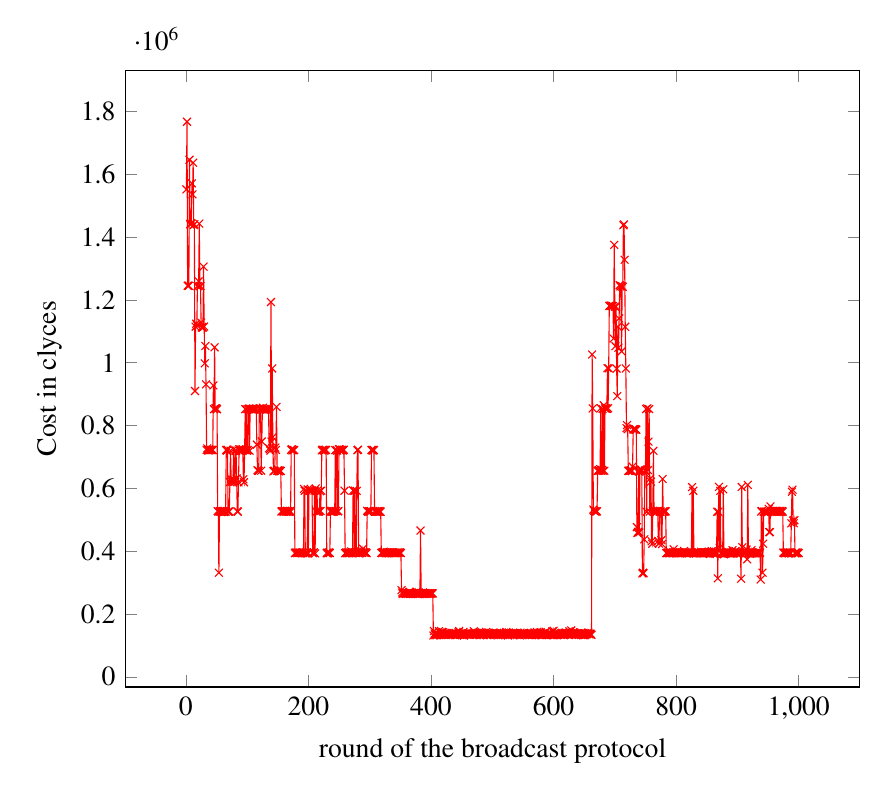
\begin{tikzpicture}
    \begin{axis}[
      xlabel=round of the broadcast protocol,
      ylabel=Cost in clyces]
    \addplot[color=red,mark=x] coordinates {
      (1,1551986)
      (2,1767396)
      (3,1245103)
      (4,1245218)
      (5,1245153)
      (6,1646349)
      (7,1440759)
      (8,1443429)
      (9,1442761)
      (10,1571085)
      (11,1536129)
      (12,1636917)
      (13,1438167)
      (14,1440759)
      (15,910123)
      (16,1114930)
      (17,1124375)
      (18,1119390)
      (19,1243732)
      (20,1244306)
      (21,1259213)
      (22,1443211)
      (23,1243931)
      (24,1243979)
      (25,1128069)
      (26,1112171)
      (27,1114456)
      (28,1111746)
      (29,1306131)
      (30,1115393)
      (31,998171)
      (32,1053532)
      (33,931168)
      (34,722147)
      (35,727529)
      (36,722582)
      (37,720077)
      (38,722550)
      (39,722833)
      (40,722295)
      (41,722271)
      (42,721841)
      (43,722681)
      (44,722120)
      (45,927799)
      (46,852087)
      (47,1049032)
      (48,854705)
      (49,854594)
      (50,854415)
      (51,851773)
      (52,528100)
      (53,526252)
      (54,331609)
      (55,525972)
      (56,527791)
      (57,525013)
      (58,527771)
      (59,526273)
      (60,526060)
      (61,527942)
      (62,524838)
      (63,528330)
      (64,526166)
      (65,526141)
      (66,722370)
      (67,720255)
      (68,723332)
      (69,525783)
      (70,526481)
      (71,526253)
      (72,620169)
      (73,720392)
      (74,629440)
      (75,621080)
      (76,626836)
      (77,619148)
      (78,723892)
      (79,627084)
      (80,621107)
      (81,720051)
      (82,719931)
      (83,631664)
      (84,527006)
      (85,526051)
      (86,619123)
      (87,724616)
      (88,718910)
      (89,723856)
      (90,719999)
      (91,719672)
      (92,722974)
      (93,724861)
      (94,628968)
      (95,619522)
      (96,721813)
      (97,852169)
      (98,721893)
      (99,852406)
      (100,720204)
      (101,722494)
      (102,852331)
      (103,854355)
      (104,719880)
      (105,853793)
      (106,852080)
      (107,851943)
      (108,851788)
      (109,852059)
      (110,854511)
      (111,850536)
      (112,852182)
      (113,851802)
      (114,853831)
      (115,851472)
      (116,739344)
      (117,658076)
      (118,655828)
      (119,655822)
      (120,854260)
      (121,853894)
      (122,854486)
      (123,656502)
      (124,749498)
      (125,852076)
      (126,856861)
      (127,850544)
      (128,852049)
      (129,852341)
      (130,852712)
      (131,852146)
      (132,850903)
      (133,851967)
      (134,852780)
      (135,852076)
      (136,727925)
      (137,724363)
      (138,720062)
      (139,1193351)
      (140,748602)
      (141,981909)
      (142,763277)
      (143,654200)
      (144,656066)
      (145,656048)
      (146,729961)
      (147,722542)
      (148,859399)
      (149,655934)
      (150,655949)
      (151,658030)
      (152,654398)
      (153,657198)
      (154,655456)
      (155,655268)
      (156,526249)
      (157,527688)
      (158,527207)
      (159,526946)
      (160,526017)
      (161,528073)
      (162,528396)
      (163,525670)
      (164,526599)
      (165,528782)
      (166,525414)
      (167,528107)
      (168,525912)
      (169,525756)
      (170,528411)
      (171,525322)
      (172,722616)
      (173,724860)
      (174,721079)
      (175,722461)
      (176,722266)
      (177,721816)
      (178,393371)
      (179,395649)
      (180,395638)
      (181,395527)
      (182,393666)
      (183,395420)
      (184,395040)
      (185,394267)
      (186,395767)
      (187,394352)
      (188,393797)
      (189,395632)
      (190,395262)
      (191,393974)
      (192,396372)
      (193,598502)
      (194,592417)
      (195,393293)
      (196,394391)
      (197,396622)
      (198,393176)
      (199,597056)
      (200,393355)
      (201,593393)
      (202,592047)
      (203,592849)
      (204,592598)
      (205,592270)
      (206,593673)
      (207,394002)
      (208,393833)
      (209,396331)
      (210,592911)
      (211,392931)
      (212,599835)
      (213,525657)
      (214,591905)
      (215,525862)
      (216,527737)
      (217,525340)
      (218,528327)
      (219,591016)
      (220,528080)
      (221,592661)
      (222,721191)
      (223,722724)
      (224,722422)
      (225,722672)
      (226,719989)
      (227,722225)
      (228,722864)
      (229,722473)
      (230,393581)
      (231,395910)
      (232,393642)
      (233,395732)
      (234,395902)
      (235,394154)
      (236,526307)
      (237,528490)
      (238,525042)
      (239,528588)
      (240,525990)
      (241,526272)
      (242,526626)
      (243,527940)
      (244,721755)
      (245,528001)
      (246,722597)
      (247,720233)
      (248,527118)
      (249,527294)
      (250,724618)
      (251,724713)
      (252,720765)
      (253,722056)
      (254,722577)
      (255,722772)
      (256,720507)
      (257,722467)
      (258,723005)
      (259,592526)
      (260,393793)
      (261,394469)
      (262,396752)
      (263,394118)
      (264,393868)
      (265,395856)
      (266,393674)
      (267,396511)
      (268,394449)
      (269,395792)
      (270,399596)
      (271,394775)
      (272,393389)
      (273,593484)
      (274,592001)
      (275,395507)
      (276,592660)
      (277,396265)
      (278,394457)
      (279,592227)
      (280,721393)
      (281,723050)
      (282,393306)
      (283,395775)
      (284,394159)
      (285,396313)
      (286,399344)
      (287,394479)
      (288,394379)
      (289,408014)
      (290,398570)
      (291,395692)
      (292,396189)
      (293,394063)
      (294,395958)
      (295,393370)
      (296,528702)
      (297,525860)
      (298,525385)
      (299,527760)
      (300,526940)
      (301,526111)
      (302,527513)
      (303,722243)
      (304,722117)
      (305,720228)
      (306,722548)
      (307,722071)
      (308,528088)
      (309,526027)
      (310,525893)
      (311,526562)
      (312,526937)
      (313,527893)
      (314,525923)
      (315,525467)
      (316,528429)
      (317,526019)
      (318,525586)
      (319,394847)
      (320,393945)
      (321,396827)
      (322,395724)
      (323,398628)
      (324,394323)
      (325,396169)
      (326,394231)
      (327,393699)
      (328,396441)
      (329,393352)
      (330,395732)
      (331,395786)
      (332,393573)
      (333,396392)
      (334,394880)
      (335,394102)
      (336,396260)
      (337,393398)
      (338,395615)
      (339,395669)
      (340,393982)
      (341,393782)
      (342,395937)
      (343,394268)
      (344,394776)
      (345,395062)
      (346,395549)
      (347,395469)
      (348,395599)
      (349,396300)
      (350,395481)
      (351,394105)
      (352,276288)
      (353,268360)
      (354,263942)
      (355,266084)
      (356,266106)
      (357,266417)
      (358,265611)
      (359,263967)
      (360,266135)
      (361,266037)
      (362,263633)
      (363,266143)
      (364,266047)
      (365,271028)
      (366,264222)
      (367,266821)
      (368,264116)
      (369,265821)
      (370,266376)
      (371,263884)
      (372,265823)
      (373,265973)
      (374,266611)
      (375,263859)
      (376,267810)
      (377,270067)
      (378,265536)
      (379,263549)
      (380,269163)
      (381,265751)
      (382,264578)
      (383,465806)
      (384,266997)
      (385,265833)
      (386,265888)
      (387,268531)
      (388,263956)
      (389,266448)
      (390,266091)
      (391,263635)
      (392,266166)
      (393,266075)
      (394,263872)
      (395,266135)
      (396,266098)
      (397,263831)
      (398,266673)
      (399,264021)
      (400,265966)
      (401,265797)
      (402,266113)
      (403,265619)
      (404,131441)
      (405,145782)
      (406,137967)
      (407,132742)
      (408,137568)
      (409,132385)
      (410,137544)
      (411,134995)
      (412,135490)
      (413,145392)
      (414,134191)
      (415,140741)
      (416,132738)
      (417,140491)
      (418,143171)
      (419,136181)
      (420,142522)
      (421,133230)
      (422,137823)
      (423,137848)
      (424,132800)
      (425,136230)
      (426,138207)
      (427,140045)
      (428,135412)
      (429,133586)
      (430,133678)
      (431,135866)
      (432,137752)
      (433,135021)
      (434,135326)
      (435,140484)
      (436,137984)
      (437,135888)
      (438,135112)
      (439,132976)
      (440,137832)
      (441,139194)
      (442,133170)
      (443,132852)
      (444,135689)
      (445,142536)
      (446,146084)
      (447,133724)
      (448,133826)
      (449,135619)
      (450,138459)
      (451,133221)
      (452,137814)
      (453,143243)
      (454,131406)
      (455,137837)
      (456,135347)
      (457,135233)
      (458,138631)
      (459,135471)
      (460,138117)
      (461,135984)
      (462,138500)
      (463,138107)
      (464,133504)
      (465,135700)
      (466,137981)
      (467,135372)
      (468,135584)
      (469,138005)
      (470,145255)
      (471,133377)
      (472,141463)
      (473,133919)
      (474,135675)
      (475,135467)
      (476,138284)
      (477,137858)
      (478,140988)
      (479,133134)
      (480,132747)
      (481,140422)
      (482,140192)
      (483,136529)
      (484,140714)
      (485,135530)
      (486,132788)
      (487,139906)
      (488,137955)
      (489,135236)
      (490,142963)
      (491,135621)
      (492,132712)
      (493,140196)
      (494,134021)
      (495,140317)
      (496,132992)
      (497,135549)
      (498,137955)
      (499,136155)
      (500,138578)
      (501,136111)
      (502,133542)
      (503,140248)
      (504,134736)
      (505,138764)
      (506,135924)
      (507,138559)
      (508,138332)
      (509,135366)
      (510,132164)
      (511,137959)
      (512,136197)
      (513,140614)
      (514,133159)
      (515,135874)
      (516,138651)
      (517,135984)
      (518,132944)
      (519,140520)
      (520,135836)
      (521,133244)
      (522,138383)
      (523,142826)
      (524,133839)
      (525,137744)
      (526,131791)
      (527,141105)
      (528,138179)
      (529,135810)
      (530,135623)
      (531,135851)
      (532,138010)
      (533,136196)
      (534,140309)
      (535,132957)
      (536,139571)
      (537,139225)
      (538,137879)
      (539,135608)
      (540,132791)
      (541,138337)
      (542,139497)
      (543,133988)
      (544,135671)
      (545,132070)
      (546,140428)
      (547,135008)
      (548,133099)
      (549,136058)
      (550,138703)
      (551,135978)
      (552,140272)
      (553,137680)
      (554,133450)
      (555,135480)
      (556,136017)
      (557,138091)
      (558,136577)
      (559,133494)
      (560,137861)
      (561,138316)
      (562,132970)
      (563,135564)
      (564,137418)
      (565,132873)
      (566,138666)
      (567,135881)
      (568,134317)
      (569,141502)
      (570,133184)
      (571,133126)
      (572,135941)
      (573,142684)
      (574,133493)
      (575,135774)
      (576,133511)
      (577,140413)
      (578,136106)
      (579,142329)
      (580,133283)
      (581,132885)
      (582,138584)
      (583,135437)
      (584,136124)
      (585,139966)
      (586,137498)
      (587,143540)
      (588,133983)
      (589,133134)
      (590,136484)
      (591,138433)
      (592,135581)
      (593,135388)
      (594,138070)
      (595,133404)
      (596,133565)
      (597,133309)
      (598,144946)
      (599,132782)
      (600,146583)
      (601,132642)
      (602,133503)
      (603,136229)
      (604,136751)
      (605,138357)
      (606,133391)
      (607,134050)
      (608,133596)
      (609,138235)
      (610,135519)
      (611,135455)
      (612,138491)
      (613,135789)
      (614,140306)
      (615,137602)
      (616,133101)
      (617,132681)
      (618,140323)
      (619,135363)
      (620,140835)
      (621,140404)
      (622,136298)
      (623,134220)
      (624,133433)
      (625,136534)
      (626,145021)
      (627,137915)
      (628,135681)
      (629,147809)
      (630,134059)
      (631,135355)
      (632,141746)
      (633,141197)
      (634,138099)
      (635,136030)
      (636,134085)
      (637,133245)
      (638,138417)
      (639,136067)
      (640,138746)
      (641,133269)
      (642,134529)
      (643,135781)
      (644,138414)
      (645,133280)
      (646,140201)
      (647,138199)
      (648,132591)
      (649,140049)
      (650,133176)
      (651,132912)
      (652,139210)
      (653,135598)
      (654,135838)
      (655,136090)
      (656,140002)
      (657,140830)
      (658,136058)
      (659,135396)
      (660,138023)
      (661,135414)
      (662,133740)
      (663,1026169)
      (664,854499)
      (665,532653)
      (666,528872)
      (667,528235)
      (668,526198)
      (669,526423)
      (670,527208)
      (671,526966)
      (672,655777)
      (673,656317)
      (674,658576)
      (675,655903)
      (676,661514)
      (677,855341)
      (678,655918)
      (679,658735)
      (680,852876)
      (681,656096)
      (682,864604)
      (683,656146)
      (684,854851)
      (685,854291)
      (686,854789)
      (687,853247)
      (688,982788)
      (689,854965)
      (690,982355)
      (691,1181054)
      (692,1181013)
      (693,1181096)
      (694,1181804)
      (695,1180865)
      (696,1180632)
      (697,1180197)
      (698,1077181)
      (699,1375422)
      (700,1178564)
      (701,1052810)
      (702,1178650)
      (703,981169)
      (704,893790)
      (705,1114913)
      (706,1048042)
      (707,1141175)
      (708,1247414)
      (709,1242816)
      (710,1244669)
      (711,1035955)
      (712,1243160)
      (713,1241750)
      (714,1437730)
      (715,1440607)
      (716,1327845)
      (717,1114572)
      (718,981837)
      (719,791891)
      (720,801422)
      (721,788277)
      (722,656044)
      (723,655839)
      (724,656233)
      (725,656380)
      (726,656409)
      (727,658025)
      (728,655224)
      (729,669512)
      (730,787919)
      (731,787673)
      (732,788837)
      (733,788224)
      (734,787893)
      (735,786738)
      (736,476733)
      (737,458017)
      (738,461693)
      (739,653754)
      (740,459770)
      (741,654049)
      (742,661223)
      (743,655811)
      (744,658707)
      (745,328992)
      (746,331401)
      (747,329756)
      (748,437896)
      (749,655983)
      (750,657492)
      (751,852665)
      (752,525505)
      (753,854773)
      (754,658295)
      (755,748930)
      (756,852452)
      (757,526189)
      (758,631411)
      (759,621364)
      (760,431804)
      (761,423618)
      (762,528696)
      (763,719639)
      (764,526063)
      (765,528180)
      (766,525013)
      (767,526601)
      (768,526765)
      (769,526287)
      (770,528384)
      (771,432924)
      (772,424378)
      (773,525932)
      (774,525918)
      (775,526213)
      (776,435432)
      (777,422660)
      (778,629948)
      (779,526384)
      (780,526235)
      (781,525585)
      (782,527922)
      (783,526631)
      (784,393973)
      (785,393850)
      (786,396114)
      (787,395606)
      (788,393442)
      (789,395826)
      (790,393601)
      (791,396045)
      (792,395204)
      (793,394562)
      (794,393194)
      (795,396405)
      (796,406200)
      (797,395701)
      (798,395288)
      (799,394032)
      (800,394099)
      (801,394745)
      (802,396388)
      (803,393545)
      (804,396314)
      (805,393948)
      (806,394518)
      (807,396214)
      (808,393627)
      (809,395969)
      (810,393674)
      (811,396183)
      (812,395868)
      (813,400755)
      (814,395194)
      (815,396455)
      (816,393835)
      (817,396084)
      (818,393215)
      (819,395714)
      (820,395589)
      (821,393249)
      (822,395745)
      (823,395861)
      (824,394528)
      (825,394626)
      (826,604255)
      (827,393666)
      (828,592373)
      (829,393069)
      (830,395374)
      (831,393773)
      (832,393952)
      (833,393312)
      (834,394368)
      (835,393882)
      (836,396380)
      (837,395958)
      (838,393565)
      (839,393760)
      (840,393999)
      (841,398111)
      (842,395296)
      (843,393891)
      (844,396468)
      (845,393186)
      (846,397229)
      (847,393841)
      (848,396321)
      (849,394368)
      (850,396028)
      (851,395959)
      (852,396312)
      (853,392809)
      (854,398260)
      (855,391321)
      (856,395354)
      (857,395413)
      (858,400466)
      (859,396117)
      (860,393489)
      (861,393320)
      (862,399942)
      (863,391951)
      (864,394732)
      (865,393441)
      (866,393696)
      (867,525710)
      (868,313583)
      (869,525735)
      (870,605038)
      (871,410952)
      (872,592114)
      (873,393580)
      (874,393101)
      (875,396104)
      (876,391753)
      (877,596957)
      (878,390059)
      (879,392208)
      (880,393784)
      (881,393948)
      (882,393534)
      (883,400544)
      (884,393385)
      (885,393946)
      (886,394596)
      (887,393636)
      (888,395035)
      (889,392314)
      (890,396094)
      (891,393483)
      (892,403276)
      (893,393269)
      (894,394747)
      (895,393767)
      (896,398352)
      (897,400693)
      (898,396231)
      (899,393655)
      (900,393641)
      (901,396322)
      (902,396875)
      (903,394055)
      (904,395661)
      (905,393068)
      (906,312394)
      (907,604595)
      (908,412653)
      (909,394297)
      (910,395312)
      (911,393504)
      (912,393919)
      (913,393500)
      (914,394108)
      (915,405663)
      (916,374158)
      (917,611154)
      (918,393609)
      (919,393722)
      (920,392763)
      (921,395524)
      (922,393221)
      (923,403524)
      (924,393604)
      (925,393827)
      (926,394525)
      (927,393687)
      (928,393948)
      (929,393469)
      (930,394276)
      (931,395748)
      (932,391922)
      (933,396037)
      (934,396058)
      (935,396290)
      (936,393235)
      (937,395641)
      (938,309923)
      (939,526414)
      (940,528054)
      (941,331707)
      (942,423942)
      (943,525840)
      (944,525493)
      (945,525284)
      (946,526134)
      (947,525596)
      (948,525410)
      (949,525928)
      (950,524289)
      (951,534857)
      (952,460973)
      (953,460767)
      (954,542540)
      (955,527694)
      (956,525886)
      (957,525551)
      (958,527892)
      (959,527147)
      (960,525970)
      (961,526197)
      (962,528589)
      (963,528114)
      (964,524649)
      (965,528495)
      (966,526498)
      (967,525469)
      (968,527981)
      (969,525633)
      (970,528559)
      (971,525856)
      (972,525652)
      (973,528096)
      (974,525921)
      (975,395465)
      (976,393834)
      (977,395731)
      (978,393105)
      (979,395493)
      (980,394193)
      (981,395600)
      (982,393533)
      (983,396306)
      (984,392981)
      (985,395295)
      (986,395978)
      (987,393120)
      (988,488906)
      (989,589366)
      (990,596005)
      (991,497328)
      (992,489300)
      (993,498813)
      (994,393499)
      (995,396060)
      (996,393676)
      (997,393960)
      (998,396079)
      (999,394461)
      (1000,393706)
    };
    \end{axis}
  \end{tikzpicture}
\end{figure}


\begin{itemize}
\item Move server to a core != 0
\item Use low-level UMP stuff
{
\renewcommand{\labelitemi}{\checkmark}
\item disable yielding
}
\item run several request in parallel, give them IDs, can use in the
  measurement struct. Good for everything having transactions (DB,
  transactional memory, consistency in replication systems)
\end{itemize}

%%%%%%%%%%%%%%%%%%%%%%%%%%%%%%%%%%%%%%%%%%%%%%%%%%
\section{Future work}

\begin{itemize}
\item Arguing that group communication/atomic broadcast and showing
  that we can do it well might be enough (appeal to atomic broadcasts
  as the foundation for other distributed algorithms, and the MPI
  primitives, that can/need to be mapped to group-communication (have
  a list of them) 
\item Need higher-level applications, such as:
  \begin{itemize}
  \item octopus
    \begin{itemize}
    \item higher level application?
    \end{itemize}
  \item capability system? \stefan{Ask Simon how expensive revocation
      currently is}
  \item a database with replication and consistency maintenance
    \begin{itemize}
    \item SharedDB? (buffers between operators, but no synchronization
      except for access to buffers, which are multiple writers, one
      reader)
    \item Crescando (some kind of state machine replication)
    \end{itemize}
  \end{itemize}
\item Machine model for topology aware tree
  \begin{itemize}
  \item Talked to Pravin about this a bit
  \end{itemize}
\item MPI collectives (as in~\cite{Tu2008})
\end{itemize}

%%%%%%%%%%%%%%%%%%%%%%%%%%%%%%%%%%%%%%%%%%%%%%%%%%
\newpage
\bibliographystyle{plain}
\bibliography{defs,db,mendeley}

\label{LastPage}

\end{document}
